\documentclass[12pt,a4paper]{report}
\usepackage[margin=2cm]{geometry}
\usepackage{indentfirst}
\usepackage{mathrsfs}
\usepackage{amsthm}
\usepackage{CJKutf8}
\usepackage{amssymb}
\usepackage{amsmath}
\usepackage{import}
\usepackage{xifthen}
\usepackage{pdfpages}
\usepackage{transparent}
\usepackage{overpic}
\usepackage{setspace}
\usepackage{rotating}
\usepackage{graphicx}
\usepackage{wasysym}
\usepackage{xcolor}
\pagestyle{empty}
\newcommand{\iso}{\mathrm{iso}}
\newcommand{\esc}{\mathrm{esc}}
\newcommand{\oversim}[1]{\parbox[t][-18pt][c]{10pt}{\scriptsize$\sim$}\hspace*{-12pt}{#1}}
\newcommand{\bbar}[1]{\overline{#1}}
\newcommand{\ul}[1]{\underline{#1}}
\newcommand{\SOL}{\fbox{ \tt s\parbox[b][2pt][c]{6pt}{o}\hspace*{-7pt} L:}}
\newcommand{\sixedge}{\mbox{\parbox[t][-2pt][c]{10pt}{\scriptsize$\blacktriangledown\hspace{-3.6pt}\blacktriangle\hspace{-4pt}\blacktriangledown$}\hspace{-10.2pt}\parbox[b][10.7pt][c]{10pt}{\scriptsize$\blacktriangle\hspace{-3.6pt}\blacktriangledown\hspace{-3.6pt}\blacktriangle$}}}
\newcommand{\indecate}{\mbox{\begin{turn}{65.9}
$>$
\end{turn}\hspace{-10.5pt}\parbox[t][-5pt][c]{10pt}{$\bot$}\hspace{-4.35pt}\parbox[t][-3.4pt][c]{4pt}{$\shortmid$}}}
\newcommand{\incfig}[1]{%
\import{./picture/}{#1.pdf_tex}
}

\begin{document}
\begin{center}
\Huge    \textbf{Group 7 Note of Planar Statistical Physics and Bernoulli Percolation}
\end{center}
\begin{center}
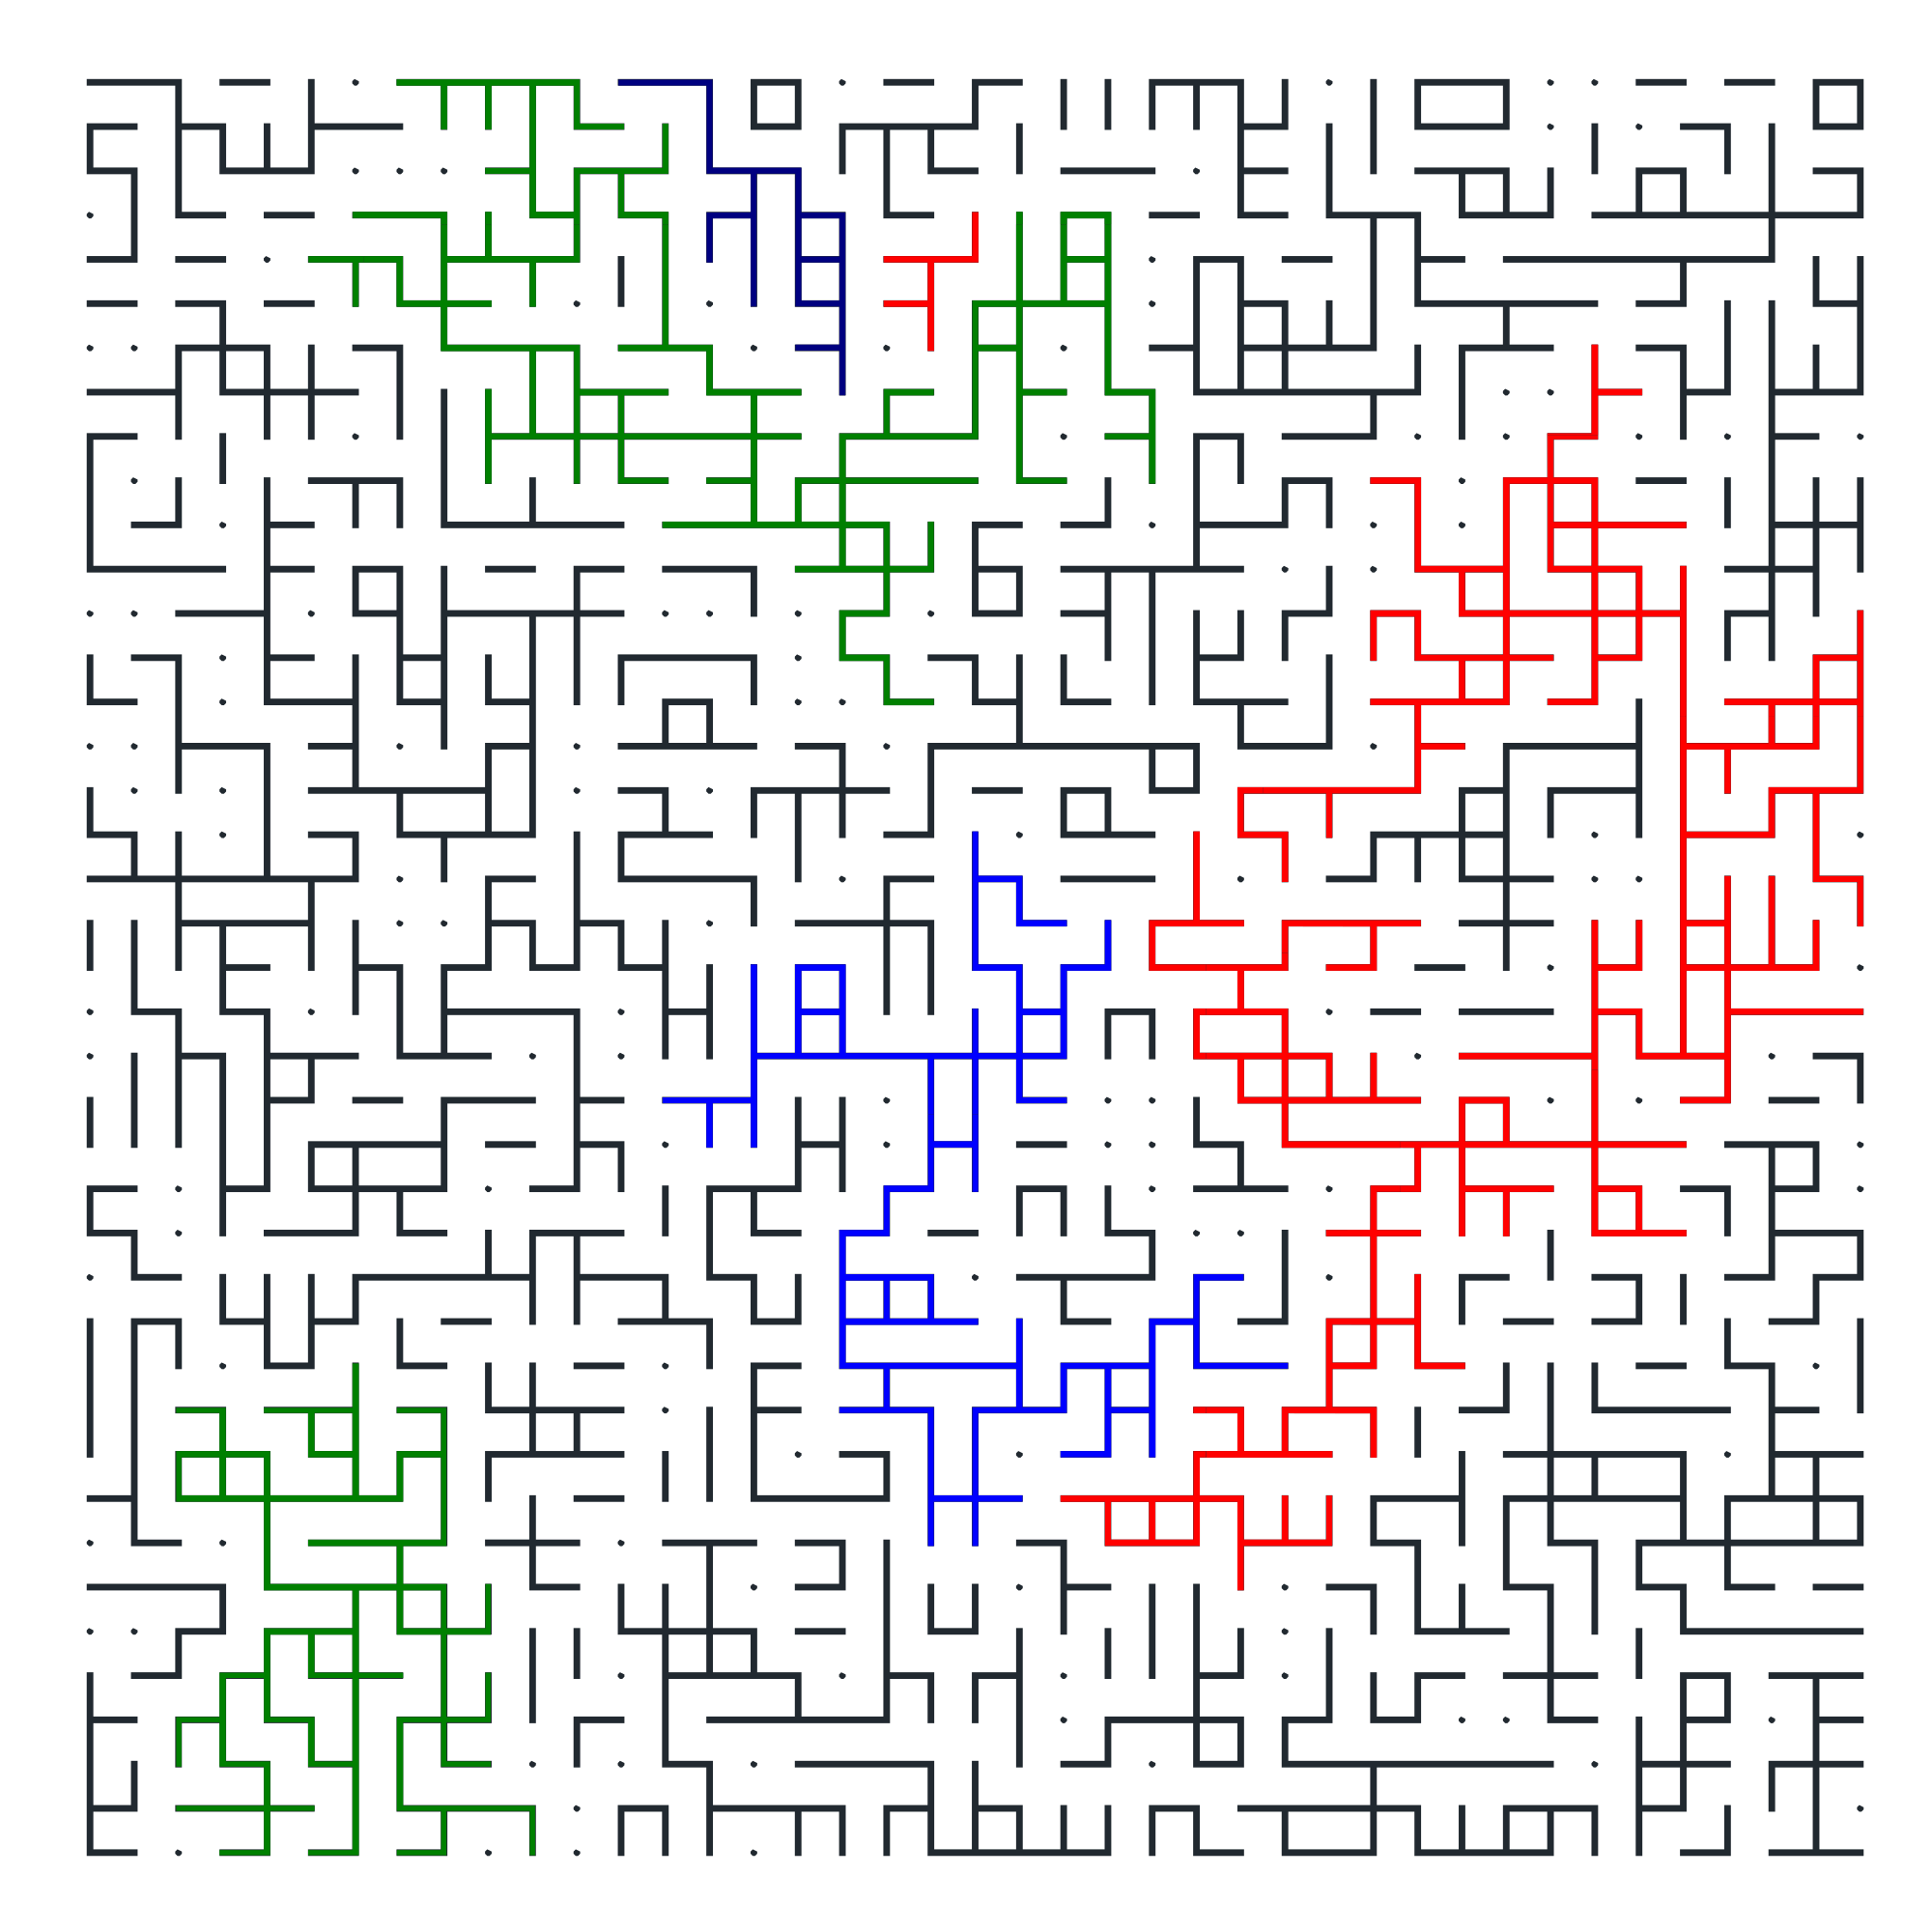
\includegraphics[width=15cm]{./picture/p=0.45.png}
\end{center}
\vspace{2cm}
\begin{flushleft}
    \begin{CJK}{UTF8}{bkai}
    學生:
    \begin{enumerate}
        \item[•] 洪偉傑
        \item[•] 郝嘉誠
        \item[•] 蘇彥維
        \item[•] 蘇士紘
        \item[•] 徐樂融
    \end{enumerate}
    \end{CJK}
\end{flushleft}
\setcounter{chapter}{-1}
\chapter{(Planer) Statistical Mechanics}
\section{Motivation}
\begin{enumerate}
    \item[•] We want to describe the (macroscopic) behavior of a system composed of huge number of (microscopic) particles. Theoretically, if the behavior of each particle can be described, then one should be able to say something about the system. However, the number of particles are astronomical (1 mole $\approx 10^{23}$) and it is costly (even impossible) to solve the system.
    \item[•] Boltzmann (end $19^{th}$ century ) gives a probabilistic formalism
    \begin{enumerate}
        \item $\Omega=$ sample space (discrete, countable, possibly infinite)
        \item $H:\Omega\to\mathbb{R}$ energy function (Hamiltonian) 
        \item $\beta=\frac{1}{T}$ inverse temperature.
    \end{enumerate}
    $\Rightarrow$ \textbf{Boltzmann distribution} 
    \[
    \mathbb{P}_{\beta}(\omega)=\frac{1}{z_\beta}\exp(-\beta H(\omega))
    \]
    Where $z_\beta=\sum\limits_{\omega\in\Omega}\exp(-\beta H(\omega))$ is called \textbf{partition function} 
    \item[•] Interpretations
    \begin{enumerate}
        \item[$*$)] At a fixed temperature, an exponential weight is associated to each configuration
        \item[$*$)] At high temperature ($\beta\to 0^+$) the weights are almost a constant function of configurations, so each state equiprobable.
        \item[$*$)] At low temperature, ($\beta\to +\infty$), the weight concentrate on minimizers of the energy function $H.$ 
    \end{enumerate}
    $\Rightarrow$ this corresponds to the intuitions we have in physics (thermodynamics?)
    \newpage
    \item[\textbf{Remark}] \begin{enumerate}
        \item $z_\beta<\infty$ if $\Omega$ is finite, so $\mathbb{P}_\beta$ is well defined.
        \item If $\Omega$ is infinite, then $z_\beta$ is not always finite. The finiteness of $z_\beta$ may depend on $\beta.$
    \end{enumerate}
\end{enumerate}
\newpage
\section{First Model (Polymer Model)}
\begin{enumerate}
	\item[•] Regular lattices, e.g., $\mathbb{Z}^d$
	\item[•] Self-avoiding walk (SAW) (a polymer)
	\begin{figure}[htp]
	\centering
	\def\svgwidth{7cm}
	\incfig{SAW1}
	\end{figure}
	\item[•] Consider $\Omega=\{\mbox{ all SAWs } \},$ define $H(\omega)=|\omega|$ where $\omega\in\Omega$\\
	Let $n\in \mathbb{N},$ define $\lambda_n=\#$ SAWs of length $n.$
	\item[\underline{Observe} : ] Given $n,m\geq 1$\\
	Any SAW of length $n+m$ can be decomposed into 2 SAWs of length $n$ and $m.$\\
	$\Rightarrow \lambda_{n+m}\leq \lambda_n\cdot \lambda_m.$
	\begin{figure}[htp]
	\centering
	\def\svgwidth{7cm}
	\incfig{SAW2}
	\end{figure}
	\item[\textbf{Exercise 1}] $\mu\equiv \lim\limits_{n\to\infty}(\lambda_n)^{\frac{1}{n}}$ exists and $\lambda_N\geq \mu^N$ for all $N\geq 1.$ $\mu$ is called the \textbf{connective constant} \\[3pt](of the graph)
	\item[\SOL] Note that $\forall n\in \mathbb{N},$ we have $(\lambda_n)^{\frac{1}{n}}\geq 0,$ thus $0$ is a lower bound of $\{(\lambda_n)^{\frac{1}{n}}\}_{n=0}^\infty,$ therefore
	\[
	\inf_{n\in\mathbb{N}_0}(\lambda_n)^{\frac{1}{n}}=K\in\mathbb{R}
	\]
	Now, given $\varepsilon>0,\ 1^{\circ}\ \exists N_1\in\mathbb{N}$ s.t.
	\[
	K+\frac{\varepsilon}{2}>(\lambda_{N_1})^\frac{1}{N_1}
	\]
	$2^{\circ}$ By division algorithm, $\forall n\geq N_1,\ \exists m,\ell \in \mathbb{Z}$ with $0\leq \ell\leq N_1$ such that $n=mN_1+\ell$, thus
	\begin{align*}
	\lambda_n=\lambda_{mN_1+\ell}\leq (\lambda_{N_1})^m\cdot \lambda_\ell
	\end{align*}
	therefore,
	\begin{align*}
	(\lambda_n)^{\frac{1}{n}}&\leq (\lambda_{N_1})^{\frac{m}{n}}\cdot (\lambda_\ell)^{\frac{1}{n}}=(\lambda_{N_1})^{\cfrac{1}{N_1+\frac{\ell}{m}}}\cdot (\lambda_\ell)^\frac{1}{n}\leq (\lambda_{N_1})^\frac{1}{N_1}\cdot (\lambda_\ell)^\frac{1}{n}\\
	&\leq (\lambda_{N_1})^\frac{1}{N_1}\cdot (\lambda_1)^\frac{\ell}{n}\leq (\lambda_{N_1})^\frac{1}{N_1}\cdot (\lambda_1)^\frac{N_1}{n}
	\end{align*}
	Because of $\lim\limits_{n\to\infty}(\lambda_{N_1})^{\frac{1}{N_1}}\cdot (\lambda_1)^{\frac{N_1}{n}}=(\lambda_{N_1})^\frac{1}{N_1},\ \exists N\in\mathbb{N}$ such that $n\geq N\Rightarrow$
	\[
	(\lambda_{N_1})^\frac{1}{N_1}+\frac{\varepsilon}{2}>(\lambda_{N_1})^\frac{1}{N_1}\cdot (\lambda_1)^{\frac{N_1}{n}}\geq (\lambda_n)^{\frac{1}{n}}
	\]
	Therefore 
	\[
	K+\varepsilon=K+\frac{\varepsilon}{2}+\frac{\varepsilon}{2}>\lambda_{N_1}^{\frac{1}{N_1}}+\frac{\varepsilon}{2}>(\lambda_n)^{\frac{1}{n}}\geq K.
	\]
	Thus, $\mu=\lim\limits_{n\to\infty}(\lambda_n)^\frac{1}{n}=K$ exists.\\
	Next, for $N>1,$ we have $\forall n\in \mathbb{N}, \lambda_{nN}\leq (\lambda_N)^n,$ thus $(\lambda_{nN})^\frac{1}{nN}\leq (\lambda_N)^\frac{1}{N}.$ Note that $\{(\lambda_{nN})^{\frac{1}{nN}}\}_{n=1}^{\infty}$ is a subsequence of $\{(\lambda_{n})^{\frac{1}{n}}\}_{n=1}^{\infty},$ therefore $\mu=\lim\limits_{n\to\infty}(\lambda_{nN})^\frac{1}{nN}\leq (\lambda_N)\frac{1}{N}\quad \blacksquare$
	\item[\textbf{Exercise 2}] \begin{enumerate}
		\item In $\mathbb{Z}^2,\ \mu\in (2,3)$
		\item In $\mathbb{Z}^3,\ \mu>3$
		\item In the triangular mesh, $\mu>3$;
		\item In the hexagonal mesh, $\mu<2$
		\item In $\mathbb{Z}\times \{0,1\}$ ( i.e. a ladder ), $\mu=\frac{1+\sqrt{5}}{2}.$
	\end{enumerate}
	\begin{figure}[htp]
	\centering
	\def\svgwidth{15cm}
	\incfig{Ex2 meshes}
	\end{figure}
	\item[\SOL] We first show a fact : 
	\newpage
	\textbf{Fact(ratio test and root test) :} Let $\{a_n\}_{n=1}^\infty$ be a sequence that take value in $(0,\infty).$ Then
	\[
	\lim_{n\to\infty}\frac{a_{n+1}}{a_n}=K\in\mathbb{R}\Rightarrow \lim_{n\to\infty}\sqrt[n]{a_n}=K.
	\]
	\begin{proof}
	If $\lim\limits_{n\to\infty}\cfrac{a_{n+1}}{a_n}=K\in\mathbb{R},$ then given $\varepsilon>0,$ there exists $N_1>0$ such that 
	\[
    	n\geq N_1\Rightarrow \Big|\frac{a_{n+1}}{a_n}-K\Big|<\frac{\varepsilon}{2}\Rightarrow K-\frac{\varepsilon}{2}<\frac{a_{n+1}}{a_n}<K+\frac{\varepsilon}{2}
	\]
	Note that $a_n=a_1\times \cfrac{a_2}{a_1}\times \cfrac{a_3}{a_2}\times \cdots \times \cfrac{a_n}{a_{n-1}}=a_1\times{\displaystyle \prod_{k=1}^{n-1} \frac{a_{k+1}}{a_k}}=a_1\times{\displaystyle \prod_{k=1}^{N_1-1} \frac{a_{k+1}}{a_k}}\times{\displaystyle \prod_{k=N_1}^{n-1} \frac{a_{k+1}}{a_k}}$ . \\
	Now define $\mathcal{Q}=a_1\times{\displaystyle \prod_{k=1}^{N_1-1} \frac{a_{k+1}}{a_k}}\ ,$ then $\sqrt[n]{a_n}=\sqrt[n]{\mathcal{Q}}\times {\displaystyle \prod_{k=N_1}^{n-1} \Big(\frac{a_{k+1}}{a_k}\Big)^{\frac{1}{n}}}\ , $ thus
	\begin{align*}
	    	\sqrt[n]{\mathcal{Q}}\times\Big(K-\frac{\varepsilon}{2}\Big)^{\frac{n-N_1-1}{n}}&= \sqrt[n]{\mathcal{Q}}\times{\displaystyle \prod_{k=N_1}^{n-1}\Big(K-\frac{\varepsilon}{2}\Big)^{\frac{1}{n}}}<\sqrt[n]{a_n}=\sqrt[n]{\mathcal{Q}}\times {\displaystyle \prod_{k=N_1}^{n-1} \Big(\frac{a_{k+1}}{a_k}\Big)^{\frac{1}{n}}}\\
	    	&<\sqrt[n]{\mathcal{Q}}\times{\displaystyle \prod_{k=N_1}^{n-1}\Big(K+\frac{\varepsilon}{2}\Big)^{\frac{1}{n}}}=\sqrt[n]{\mathcal{Q}}\times\Big(K+\frac{\varepsilon}{2}\Big)^{\frac{n-N_1-1}{n}}.
	\end{align*}
	By the fact that \\
	$A(n)=\sqrt[n]{\mathcal{Q}}\times\Big(K-\cfrac{\varepsilon}{2}\,\Big)^{\frac{n-N_1-1}{n}}\to K-\cfrac{\varepsilon}{2}\ ,\ B(n)=\sqrt[n]{\mathcal{Q}}\times\Big(K+\cfrac{\varepsilon}{2}\,\Big)^{\frac{n-N_1-1}{n}}\to K+\cfrac{\varepsilon}{2} $ as\\[3pt] $n\to\infty,$ there is $N>N_1$ such that $n\geq N\Rightarrow A(n)>K-\varepsilon$ and $B(n)<K+\varepsilon,$ thus 
	\[
	K-\varepsilon<A(n)<\sqrt[n]{a_n}<B(n)<K+\varepsilon.
	\]
	Therefore, $\lim\limits_{n\to\infty}\sqrt[n]{a_n}=K.$
	\end{proof}
	\begin{enumerate}
		\item We first show that $\mu(\mathbb{Z}^2)>2:$
		\begin{figure}[htp]
		\centering
		\def\svgwidth{8cm}
		\incfig{Ex2 Z2 lowerbound}
		\end{figure}
		\newpage
		If we only consider the 3 direction $\uparrow,\rightarrow,\downarrow$ to choose for next step, ex : red line and blue line, we define $S(n)=\#$ SAWs with length $n$ that under this restriction, $n\geq 1$ and $S(0)=1.$ Now considering the samples SAWs are of length $n,$ then 
		\begin{align*}
	    	S(n)=&\#\mbox{ SAWs passing } O\mbox{ with } \rightarrow\\
	    	+\sum_{k=1}^n &\#\mbox{ SAWs passing } A_i\mbox{ with } \rightarrow + \sum_{k=1}^n \#\mbox{ SAWs passing } A_{-i}\mbox{ with } \rightarrow\\
	    	+&\#\mbox{ SAWs lying in } y\mbox{- axis}\\
	    	=& S(n-1)+2S(n-2)+\cdots +2S(1)+2S(0)+2\\
	    	=&S(n-1)+2+2\sum_{k=0}^{n-2}S(k),\quad n\geq 2
	    \end{align*}
	    Similarly, $S(n+1)=S(n)+2+2\sum\limits_{k=0}^{n-1}S(k),$ by subtraction of the two equation, we get a recursive formula :
	    \[
	    S(n+1)=2S(n)+S(n-1),\quad n\geq 1,\ \cdots\cdots(*)
	    \]
	    We get $\{S(n)\}_{n=0}^\infty:1,3,7,17,31,\cdots,$ we use matrix representation of $(*):$
	    \[
	    \begin{bmatrix}
	    S(n+1)\\
	    S(n)
	    \end{bmatrix}=\begin{bmatrix}
	    2 & 1\\
	    1 & 0
	    \end{bmatrix}\begin{bmatrix}
	    S(n)\\
	    S(n-1)
	    \end{bmatrix}.
	    \]
	    And note that by calculating eigenvalue and eigenvector, we have 
	    \begin{align*}
	    \begin{bmatrix}
	    2 & 1\\
	    1 & 0
	    \end{bmatrix}=P&\begin{bmatrix}
	    1+\sqrt{2} & 0\\
	    0 & 1-\sqrt{2}
	    \end{bmatrix}P^{-1},\quad P=\begin{bmatrix}
	    1 & -1\\
	    -1+\sqrt{2} & 1+\sqrt{2}
	    \end{bmatrix}\\
	    \Rightarrow & \begin{bmatrix}
	    2 & 1\\
	    1 & 0
	    \end{bmatrix}^n=P\begin{bmatrix}
	    (1+\sqrt{2})^n & 0\\
	    0 & (1-\sqrt{2})^n
	    \end{bmatrix}P^{-1}\\
	    \Rightarrow &\begin{bmatrix}
	    S(n+1)\\
	    S(n)
	    \end{bmatrix}=\begin{bmatrix}
	    2 & 1\\
	    1 & 0
	    \end{bmatrix}^n\begin{bmatrix}
	    S(1)\\
	    S(0)
	    \end{bmatrix}=\begin{bmatrix}
	    2 & 1\\
	    1 & 0
	    \end{bmatrix}^n\begin{bmatrix}
	    3\\
	    1
	    \end{bmatrix}\\
	    =& \frac{1}{2}P\begin{bmatrix}
	    (1+\sqrt{2})^n & 0\\
	    0 & (1-\sqrt{2})^n
	    \end{bmatrix}\begin{bmatrix}
	    4+3\sqrt{2}\\
	    4-3\sqrt{2}
	    \end{bmatrix}\\
	    =& \frac{1}{2}\begin{bmatrix}
	    1 & -1\\
	    -1+\sqrt{2} & 1+\sqrt{2}
	    \end{bmatrix}\begin{bmatrix}
	    (1+\sqrt{2})^n(4+3\sqrt{2})\\
	    (1-\sqrt{2})^n(4-3\sqrt{2})
	    \end{bmatrix}\\
	    \Rightarrow S(n+1)=& \frac{1}{2}\Big((1+\sqrt{2})^n(4+3\sqrt{2})-(1-\sqrt{2})^n(4-3\sqrt{2})\Big)
	    \end{align*}
	    Thus, $\mu(\mathbb{Z}^2)=\lim\limits_{n\to\infty}\sqrt[n+1]{\lambda_{n+1}}\geq \lim\limits_{n\to\infty}\sqrt[n+1]{S(n+1)}=1+\sqrt{2}>2.$\\[5pt]
	    Next, we show that $\mu<3:$\\
	    First, we calculate the number of SAWs of length 4 with the first move is $``\rightarrow"$
	    \newpage
		\begin{figure}[htp]
		\centering
		\def\svgwidth{8cm}
		\incfig{Ex2 Z2 upperbound}
		\end{figure}
		We got that number is 25 (blue points),this figure concentrate about the direction of next move of SAWs instead of the distance between two connected points (it is always 1). we get $\lambda_{4}=4\times 25=100$ Now we replace blue point by red point, and then we got $\lambda_7\leq \lambda_4\times 25=2500,$ continue this process, we got $\lambda_{1+3n}\leq 4\times 25^n.$ Thus 
		\[
		\mu(\mathbb{Z}^2)=\lim_{n\to\infty}(\lambda_{3n+1})^{\frac{1}{3n+1}}\leq \lim_{n\to\infty}4^{\frac{1}{3n+1}}\times 25^{\frac{n}{3n+1}}=\sqrt[3]{25}<3.
		\]
		\item Because of $\mathbb{Z}^3=\mathbb{Z}^2\times \mathbb{Z},$ thus we define $\beta_n$ be the number of SAWs of length $n$ in $\mathbb{Z}^2,$ by (a), we have $\lim\limits_{n\to\infty}\sqrt[n]{\beta_n}=\mu(\mathbb{Z}^2)\in(2,3).$ Note that $\lambda_{n+1}\geq \beta_n\times 2^{n+1},$ therefore 
		\[
		\mu(\mathbb{Z}^3)=\lim_{n\to\infty}\sqrt[n+1]{\lambda_{n+1}}\geq \lim_{n\to\infty}\sqrt[n+1]{\beta^n}\times 2^{\frac{n+1}{n+1}}\geq \lim_{n\to\infty}\Big(\frac{\beta_{n+1}}{4}\Big)^{\frac{1}{n+1}}\times 2>2\times 2>3
		\]
		\item If we look more seriously, we can find that there's a hidden $\mathbb{Z}^2$ in the triangular mesh :
		\begin{figure}[htp]
		\centering
		\def\svgwidth{6cm}
		\incfig{Ex2 triangular meshes}
		\end{figure}
		\\
		But, we are not going to use this fact. Instead, we'll prove $\mu(\triangle)>3$ by using the similar way to prove $\mu(\mathbb{Z}^2)>2.$ Define $S(n)$ be \# of SAWs with length $n$ that every move only choose the four blue directions (\textbf{Figure 1}), if we define $S(0)=1,$ it is easy to see that 
		\begin{align*}
		S(n)&=2S(n-1)+4S(n-2)+\cdots +4S(0)+2=2+2S(n-1)+4\sum_{k=0}^{n-2}S(k)\\
		S(n+1)&=2S(n)+4S(n-1)+\cdots +4S(0)+2=2+2S(n)+4\sum_{k=0}^{n-1}S(k)\quad n\geq 2.
		\end{align*}
		\newpage
		Thus, $S(n+1)-S(n)=2S(n)+2S(n-1)$\\$\Rightarrow S(n+1)=3S(n)+2S(n-1),\quad n\geq 2,\ S(0)=1,\ S(1)=4,\ S(2)=14,$ thus
		\[
		\begin{bmatrix}
		S(n+1)\\
		S(n)
		\end{bmatrix}=\begin{bmatrix}
		3 & 2\\
		1 & 0
		\end{bmatrix}\begin{bmatrix}
		S(n)\\
		S(n-1)
		\end{bmatrix}
		\]
		We note that 
		\[
		\begin{bmatrix}
		3 & 2\\
		1 & 0
		\end{bmatrix}=P\begin{bmatrix}
		\frac{3+\sqrt{17}}{2} & 0\\
		0 & \frac{3-\sqrt{17}}{2}
		\end{bmatrix}P^{-1},\quad\mbox{where }P=\begin{bmatrix}
		3+\sqrt{17} & 3-\sqrt{17}\\
		2 & 2
		\end{bmatrix}
		\]
		And
		\[
		P^{-1}=\frac{1}{4\sqrt{17}}\begin{bmatrix}
		2 & -3+\sqrt{17}\\
		-2 & 3+\sqrt{17}
		\end{bmatrix}
		\]
		Therefore,
		\begin{align*}
		    \begin{bmatrix}
		    S(n+1)\\
		    S(n)
		    \end{bmatrix}&=\begin{bmatrix}
		    3 & 2\\
		    1 & 0
		    \end{bmatrix}^n\begin{bmatrix}
		    S(1)\\
		    S(0)
		    \end{bmatrix}=P\begin{bmatrix}
    		\frac{3+\sqrt{17}}{2} & 0\\
    		0 & \frac{3-\sqrt{17}}{2}
    		\end{bmatrix}^n\hspace{-5pt} P^{-1}\begin{bmatrix}
    		4\\
    		1
    		\end{bmatrix}\\
    		&=\frac{1}{4\sqrt{17}}P\begin{bmatrix}
    		\big(\frac{3+\sqrt{17}}{2}\big)^n & 0\\
    		0 & \big(\frac{3-\sqrt{17}}{2}\big)^n
    		\end{bmatrix}\begin{bmatrix}
    		5+\sqrt{17}\\
    		-5+\sqrt{17}
    		\end{bmatrix}\\
    		&=\frac{1}{4\sqrt{17}}\begin{bmatrix}
    		3+\sqrt{17} & 3-\sqrt{17}\\
    		2 & 2
    		\end{bmatrix}\begin{bmatrix}
    		\big(\frac{3+\sqrt{17}}{2}\big)^n(5+\sqrt{17})\\[3pt]
    		\big(\frac{3-\sqrt{17}}{2}\big)^n(-5+\sqrt{17})
    		\end{bmatrix}
		\end{align*}
		Thus implies that
		\[
		S(n)=\frac{2}{4\sqrt{17}}\bigg(\Big(\frac{3+\sqrt{17}}{2}\Big)^n(5+\sqrt{17})+\Big(\frac{3-\sqrt{17}}{2}\Big)^n(-5+\sqrt{17})\bigg)
		\]
		And therefore
		\[
		\mu(\triangle)=\lim_{n\to\infty}\sqrt[n]{\lambda_n}\geq \lim_{n\to\infty}\sqrt[n]{S(n)}=\frac{3+\sqrt{17}}{2}>3.
		\]
		\item  Similar way to prove $\mu(\mathbb{Z}^2)<3,$ we use a simple calculate, deduce that 
		\[
		\lambda_{1+5}=(3\times 2^5-2)=\lambda_1\times 30
		\]
		Thus,
		\[
		\lambda_{1+5n}\leq \lambda_1\times 30^{n}
		\]
		Therefore,
		\[
		\mu(\sixedge)=\lim_{n\to\infty}\sqrt[1+5n]{\lambda_{1+5n}}\leq \lim_{n\to\infty}\sqrt[1+5n]{\lambda_1\times 30^n}=\sqrt[5]{30}<2
		\]
		\item \textit{Claim} `` $\mu(\mathbb{Z}\times\{0,1\})\geq \frac{1+\sqrt{5}}{2}$ " : \\
		Let $S(n)$ be \# of SAWs with length $n$ that only move $\uparrow,\ \downarrow,\ \rightarrow$ in every step, and it is easy to see that $S(n)=S(n-1)+S(n_2),\quad n\geq 3,$ therefore
		\[
		\mu(\mathbb{Z}\times\{0,1\})=\lim_{n\to\infty}\sqrt[n]{\lambda_n}\geq\lim_{n\to\infty}\sqrt[n]{S(n)}=\frac{1+\sqrt{5}}{2}
		\]
		\newpage
		\textit{Claim} `` $\mu(\mathbb{Z}\times\{0,1\})\leq\frac{1+\sqrt{5}}{2}$ " :\\
		Define $T(n)$ be \# of SAWs in $\mathbb{N}_0\times \{0,1\}$ of length $n$, $n\in \mathbb{N},$ and define $T(0)=1.$ You well find that recursive formula is a great way to slove these problem.
		\[
		T(n)=T(n-2)+T(n-3)+\cdots +T(0)+\gamma(n), 
		\]
		where $ \gamma(n)=\bigg\{\begin{array}[c]{l}
		\frac{n+3}{2},\quad \mbox{if } n \mbox{ is odd.}\\
		\frac{n+2}{2},\quad \mbox{if }n \mbox{ is even.}
		\end{array} $
		\begin{figure}[htp]
		\centering
		\def\svgwidth{10cm}
		\incfig{Ex2 ladder}
		\end{figure}
		We find that 
		\[
		T(n+1)-T(n)=T(n-1)+\gamma(n+1)-\gamma(n)=T(n-1)+\indecate_{even}(n),
		\]
		where $\indecate_{even}(n)=\bigg\{\begin{array}[c]{l}
		0,\quad \mbox{if } n \mbox{ is odd.}\\
		1,\quad \mbox{if }n \mbox{ is even.}
		\end{array}$\\[3pt]
		Moreover, $\lambda_n\leq 2T(n)+2(T(n-4)+T(n-6)+\cdots )$,\quad $n\in\mathbb{N}$, thus
		\begin{align*}
		    \lambda_n&\leq\lambda_n+\lambda_{n+1}\leq 2(T(n+1)+T(n))+2(T(n-3)+\cdots +T(0))\\
		    &=2(T(n+1)+T(n)+T(n-1)-\gamma(n-1))\\
		    &=2(2T(n+1)+\indecate_{even}(n)-\gamma(n))\leq 4T(n+1),\ \forall n\in\mathbb{N}
		\end{align*}
		Because of $T(0)=1,\ T(1)=2,$ and 
		\[ 
		T(n+1)\geq T(n)+T(n_1),\ T(n+1)+1\leq (T(n)+1)+(T(n-1)+1)
		\]
		Define\\
		$\{a_n\}_{n=0}^\infty$ as $a_0=1,\ a_1=2,\ a_{n+1}=a_n+a_{n-1},\quad n\geq 1$\\
		$\{b_n\}_{n=0}^\infty$ as $b_0=2,\ b_1=3,\ b_{n+1}=b_n+b_{n-1},\quad n\geq 1$, then 
		\[
		a_n\leq T(n)<T(n)+1\leq b_n,\quad \forall n\in\mathbb{N}.
		\]
		We note that both $a_n$ and $b_n$ are Fibonacci sequence, thus
		\[
		\lim_{n\to\infty}\sqrt[n]{a_n}=\lim_{n\to\infty}\sqrt[n]{b_n}=\frac{1+\sqrt{5}}{2}\Rightarrow \lim_{n\to\infty}\sqrt[n]{T(n)}=\frac{1+\sqrt{5}}{2}
		\]
		Therefore,
		\[
		\mu(\mathbb{Z}\times \{0,1\})=\lim_{n\to\infty}\sqrt[n]{\lambda_n}\leq \lim_{n\to\infty}\sqrt[n]{4T(n+1)}=\frac{1+\sqrt{5}}{2}\quad \blacksquare
		\]
	\end{enumerate}
	\item[\textbf{Remark.}] \begin{enumerate}
		\item Highly non-trivial to compute $\mu.$
		\item On the hexagonal lattice, it is shown that $\mu=\sqrt{2+\sqrt{2}}$ (2010, Copin at el.)
		\item By computer simulation,\\
		\textbf{Conjecture} : $Z_\beta=(\beta-\beta_c)^{-\gamma+o(1)}$ for $\beta\to \beta_c^+,$ where $\gamma$ only depends on that dimension of the lattice. In 2D, $\gamma=\frac{43}{32}$ (conjectured)
		\item If we have $\lambda_N\sim \mu^NN^\alpha ,$ then $Z_\beta$ can be computed to satisfy $Z_\beta\sim (\beta-\beta_c)^{-1+\alpha},$ $\alpha=\frac{11}{32}$ in 2D (conjectured) 
	\end{enumerate}
	\item[\textbf{Exercise 3}] How to sample SAWs with computer. (Think of Markov process whose invariant measure is $\mathbb{P}_\beta$)
\end{enumerate}
\newpage
\section{Bernoulli Percolation}
\begin{flushleft}
We first consider $\mathbb{Z}^d$ lattices,
\begin{enumerate}
	\item[•] \textbf{Bond percolation} Give $p\in [0,1],$ consider $\omega=(\omega(e))_{e\in\mathbb{Z}^d}$ such that $\{\omega(e)\}_{e\in\mathbb{Z}^d}$ is i.i.d with $\omega(e)\sim\mathrm{Brenoulli}(p).$\\
	If $\omega(e)=1,$ we say that $e$ is open. If $\omega(e)=0,$ we say that $e$ is closed.\\
	\textbf{Remark} We got a model of random subgraph. By above of notation, we may also write $\omega$ for the random subgraph (consisting of that open edges).
	\item[•] \textbf{Site percolation} Same thing with i.i.d $\mathrm{Bernoulli}(p),$\\
	open means that the node can pass, closed means that the node can not pass.
	\item[•] Notation : \\
	$\mathbb{P}_p=$ The Bernoulli percolation of parameter $p.$\\
	$\omega_p$ a sample of $\mathbb{P}_p$
	\begin{figure}[htp]
	\centering
	\def\svgwidth{15cm}
	\incfig{bound and site percolation}
	\end{figure}
	\item[\textbf{Remark}] The terminology ``Bernoulli percolation" stands for \textbf{i.i.d}, on the other hand, without independence, we simply say that we have a ``percolation model", e.g. random cluster model.\\
	For the following classes we use ``percolation" to refer to Bernoulli percolation.
	\item[\textbf{Exercise 1}] Show that a bond percolation is equivalent to a site percolation. How about the other way? Construct an example.
	\item[\textbf{Question :}] What are the interesting behavior when $p$ varies? e.g. \# component, size of component etc.\\
	$p=0$ is an empty graph, $p=1$ is a full graph. 
	\item[•] \textbf{Connected component (cluster)}\\
	Let $a,b$ be two vertex of $\mathbb{Z}^d,$ we say that $a\sim b$ if exists an path in $\omega_p$ from $a$ to $b$. It is clearly that $\sim$ is an equivalence relation. \\
	A \textbf{connected component}(cluster) is an element in equivalence classes of $\sim$ 
	\item[•] \textbf{Infinite cluster}\\
	A infinite cluster is a cluster of $\omega_p$ that has infinite edges and infinite vertex.\\
	Let $[O\leftrightarrow \infty]$ be the event in $\mathbb{P}_p$ that $O$ belongs to a infinite cluster.\\
	$\theta(p)=\mathbb{P}_p[O\leftrightarrow\infty].$
	\item[\textbf{Exercise 2}] Let $\mathbb{T}_d$ be a regular tree, i.e., an infinite connected graph with countably many vertices without cycles where all the vertices is of degree $d.$ \underline{Ex} : $\mathbb{T}_2=\mathbb{Z},$
	\newpage
	\begin{figure}[htp]
	\centering
	\def\svgwidth{5cm}
	\incfig{T3}
	\end{figure}
	\item[\SOL] We study $p_c$ of $\mathbb{T}_d,\ d\geq 2.$\\
	If $d=2,$ i.e., $\mathbb{T}_2=\mathbb{Z},$ consider 
	\begin{align*}
	\beta(p):=\mathbb{P}_p[O\leftrightarrow\infty\mbox{ in }\mathbb{N}_0]&=1-(1-p)-p(1-p)-p^2(1-p)-\cdots\\
	&=1-\frac{1-p}{1-p}=0,\quad \mbox{ if } p\neq 1.\\
	&=1,\ \, \qquad\qquad\qquad \mbox{ if }p=1.
	\end{align*}
	Then, $\theta(p)=2\beta(p)-\beta(p)^2=\beta(p).$
	Thus, $p_c(\mathbb{T}_2)=\sup\{p\mid \theta(p)=0\}=1.$\\[4pt]
	If $d=3,$ consider $\mathbb{I}_3\subseteq \mathbb{T}_3$ and define $\beta(p)=\mathbb{P}_p[O\leftrightarrow\infty\mbox{ in }\mathbb{I}_3].$
	\begin{figure}[htp]
	\centering
	\def\svgwidth{5cm}
	\incfig{I3}
	\end{figure}\\
	Then,
	\[
	\beta(p)=2p\beta(p)-p^2\beta(p)^2\Rightarrow \beta(p)=0\mbox{ or }\frac{2p-1}{p^2}.
	\]
	Because of $\beta(p)\geq 0$ for all $p\in [0,1],$ we get $\beta(p)=0$ if $p\in [0,\frac{1}{2}].$\\
	On the other hand, we use a similar way of $d=2$ to calculate $\beta(p):$
	\[
	\beta(p)=1-\sum_{n=0}^\infty a_np^n(1-p)^{n+2}=1-(1-p)^2\sum_{n=0}^\infty a_np^n(1-p)^n
	\]
	where $a_n=\#$ of $n$-edges clusters in $\mathbb{I}_2$ that contains $O.$\\
	If $p\in [0,\frac{1}{2}],$ then $\beta(p)=0,$ thus 
	\[
	\sum_{n=0}^\infty a_np^n(1-p)^n=\frac{1}{(1-p)^2}
	\]
	Therefore, if $p\in [\frac{1}{2},1],$ we get $1-p\in[0,\frac{1}{2}],$ and thus
	\[
		\sum_{n=0}^\infty a_np^n(1-p)^n=\sum_{n=0}^\infty a_n(1-p)^n(1-(1-p))^n=\frac{1}{p^2}
	\]
	Thus,
	\[
	\beta(p)=1-\frac{(1-p)^2}{p^2}=\frac{2p-1}{p^2}
	\]
	And we can calculate $\theta(p)=\beta(p)+p\beta(p)-p\beta(p)^2,$ and find that
	\[
	p_c(\mathbb{T}_3)=\sup\{p\mid \theta(p)=0\}=\sup\{p\mid \beta(p)=0\}=\frac{1}{2}
	\]
	For a general $d\geq 3,$ and still studying $p_c(\mathbb{T}_d),$ still consider $\mathbb{I}_d\subseteq \mathbb{T}_d$ be a connected graph that the degree of $O$ is $d-1$ and is $d$ in other vertices. 
	\begin{enumerate}
	    \item[$1^\circ$] Consider 
	\[
	\beta(p)=\mathbb{P}_p[O\leftrightarrow\infty\mbox{ in }\mathbb{I}_d],
	\]
	then $1-\beta(p)=(1-p\beta(p))^{d-1}.$ Now, consider the case that $p=\frac{1}{d-1},$ then
	\[
	1-\beta\Big(\frac{1}{d-1}\Big)=\bigg(1-\frac{1}{d-1}\beta\Big(\frac{1}{d-1}\Big)\bigg)^{d-1},\quad \mbox{let }u=1-\frac{1}{d-1}\beta\Big(\frac{1}{d-1}\Big),
	\]
	we get 
	\[
	-d+2+(d-1)u=u^{d-1}\cdots\cdots (*)
	\]
	Because of $0\leq \beta(\frac{1}{d-1})\leq 1,$ we have $1-\frac{1}{d-1}\leq u\leq 1,$ we know that if $0<u<1,$ then $u^{d-1}-(d-1)u=u(u^{d-2}-(d-1))>u^{d-2}-d+1>-d+2,$ thus the solution of $(*)$ is $u=1,$ and thus $\beta(\frac{1}{d-1})=0.$ Remark that
	\[
	\theta(p)=\beta(p)+p\beta(p)-p\beta(p)^2,
	\]
	thus $\theta(\frac{1}{d-1})=0,$ thus $p_c\geq \frac{1}{d-1}.$
	\item[$2^\circ$] Note that
	\[
	\beta(p)=1-\sum_{n=0}^\infty a_np^n(1-p)^{(d-2)n+d-1}=1-(1-p)^{d-1}\sum_{n=0}^\infty a_np^n(1-p)^{(d-2)n}
	\]
	where $a_n=\#$ of $n$-edges clusters in $\mathbb{I}_d$ that contain $O.$\\
	We consider the polynomial $f(p)=p(1-p)^{d-2},$ we have $f(0)=f(1)=0,$ and $f(p)\geq 0$ if $p\in [0,1].$ Note that
	\[
	f'(p)=(1-p)^{d-2}-(d-2)p(1-p)^{d-3}=(1-p)^{d-3}\big[1-(d-1)p\big]
	\]
	Thus, critical points of $f$ on $[0,1]$ is $0,\ 1, \ \frac{1}{d-1},$ thus $f(\frac{1}{d-1})$ is the maximal value in $[0,1].$ Thus, if $p\in(\frac{1}{n-1},1]$
	\begin{align*}
	\beta(p)&=1-(1-p)^{d-1}\sum_{n=0}^\infty a_nf(p)^n\\
	&\geq 1-(1-p)^{d-1}\sum_{n=0}^\infty a_nf\big(\frac{1}{n-1}\big)^n \\
	&> 1-\big(1-\frac{1}{d-1}\big)^{d-1}\sum_{n=0}^\infty a_nf\big(\frac{1}{n-1}\big)^n\\
	&=\beta\big(\frac{1}{n-1}\big)=0.
	\end{align*}
	Thus, $p_c(\mathbb{T}_d)=\frac{1}{1-d},\ d\geq 2$\qquad $\blacksquare$
	\end{enumerate}
	\item[\textbf{Exercise 3}] Define the random-cluster model and discuss the following :
	\begin{enumerate}
	    \item[(a)] Why it can only be defined on a finite graph?
	    \item[(b)] The heuristic behavior of the model when $\female$ varies.\\
	    ( $\female\to 0^+$\quad UST,\\ $\female=1$ Bernoulli percolation, \\
	    $\female>1$ configurations with more clusters are preferred\\
	    $\female<1$ configurations with less clusters are preferred)
	    \item[(c)] The definition of the model is ``global", i.e., one needs to count the number of clusters so needs to know where a configuration looks like in the \underline{whole} graph.
	    \item[(d)] For a planer random-cluster model, the FK-loop representation makes the definition ``local". (This may be hard to discuss at the moment)
	\end{enumerate}
\end{enumerate}
\end{flushleft}
\newpage
\chapter{Basic Properties of the Bernoulli Percolation}
\begin{flushleft}
	Consider $G=\mathbb{Z}^d$ or some ``nice" graph.\\[1cm]
\end{flushleft}

\section{Coupling \begin{CJK}{UTF8}{bkai}(耦合)\end{CJK}}
\begin{enumerate}
	\item[•] Given $p\leq p',$ how to compute $X\sim \mathrm{Bernoulli}(p),\ X'\sim\mathrm{Bernoulli}(p')$?\\
	Consider $\mathcal{U}\sim\mathrm{Uniform}([0,1]),$ define $Y=\mathbf{1}_{\, \mathcal{U}\leq p},$ $Y'=\mathbf{1}_{\, \mathcal{U}\leq p'}$, we get 
	\[
	X\overset{(id)}{=}Y,\quad X'\overset{(id)}{=}Y',\quad Y\leq Y'.\quad a.s. (almost\ sure)
	\]
	This is called a coupling.
	\item[\textbf{Remark.}] In coupling, usually we do not want independence, so that we can compute values between random variables.
	\item[\textbf{Exercise 1}] Construct a coupling between $\omega\sim\mathbb{P}_p,\ \omega'\sim\mathbb{P}_{p'}$ with $p\leq p',$ so that values between edges can be computed.\\
	Wanted : $p\leq p'\Rightarrow \omega_p\leq \omega_p'(\Leftrightarrow \omega_p(e)\leq \omega_{p'}(e),\ \forall e\in E)$
	\item[\SOL] Let $\omega=(\omega(e))_{e\in G}$ such that $\{\omega(e)\}_{e\in G}$ is i.i.d. and $\omega(e)\sim \mathrm{Uniform}([0,1]).$ \\
	Define $\omega_p\sim\mathbb{P}_p,\ \omega_{p'}\sim\mathbb{P}_{p'}$ as $\forall e\in E,\ \omega_p(e)=\mathbf{1}_{\omega(e)\leq p},\ \omega_{p'}(e)=\mathbf{1}_{\omega(e)\leq p'},$ thus, $p\leq p'\Rightarrow \forall e\in E,\ \omega_p(e)\leq \omega_{p'}(e).$
	\item[\textbf{Exercise 2}] Given $O\in V(G),$ define $\theta:\begin{array}[t]{ccl}
	[0,1]&\to&\mathbb{R}\\
	p&\mapsto&\mathbb{P}_p([O\leftrightarrow\infty])
	\end{array}	 $ (percolation function).\\
	Show that $\theta$ is increasing. In more general case, at must how many different $\theta$ function can be obtain?
	\item[\SOL] If $p\leq p',$ let $\omega_1\sim \mathbb{P}_p,\ \omega_2\sim \mathbb{P}_{p'},$ we use the definition of \textbf{Exercise 1}, we have\\ $\omega_1\overset{(id)}{=}\omega_p,\ \omega_2\overset{(id)}{=}\omega_{p'},$ thus $\mathbb{P}_p([O\leftrightarrow\infty])=\mathbb{P}_p([O\leftrightarrow\infty]\mbox{ in }\omega_1)=\mathbb{P}_p([O\leftrightarrow\infty]\mbox{ in }\omega_p),$ 
	\newpage
	similarly, $\mathbb{P}_{p'}([O\leftrightarrow\infty])=\mathbb{P}_{p'}([O\leftrightarrow\infty]\mbox{ in }\omega_1)=\mathbb{P}_{p'}([O\leftrightarrow\infty]\mbox{ in }\omega_{p'}).$ We note that $\omega_p$ is always a subgraph of $\omega_{p'}$ (by \textbf{Exercise 1}), thus $\{[O\leftrightarrow\infty]\mbox{ in }\omega_p\}\subseteq\{[O\leftrightarrow\infty]\mbox{ in }\omega_{p'}\},$ we have $\mathbb{P}_p([O\leftrightarrow\infty])=\mathbb{P}_p([O\leftrightarrow\infty]\mbox{ in }\omega_p)\leq \mathbb{P}_{p'}([O\leftrightarrow\infty]\mbox{ in }\omega_{p'})=\mathbb{P}_{p'}([O\leftrightarrow\infty]).$\\
	And, because of $\omega_1\overset{(id)}{=}\omega_p,$ where $\omega_1$ is a arbitrary random variable with $\omega_1\sim\mathbb{P}_p$ thus there are only one choice of $\theta.$ i.e., $\theta$ is well-defined. $\blacksquare$
	\item[•] Define $p_c=\sup\{p\in [0,1]\,|\,\theta(p)=0\}$
	\item[\textbf{Exercise 3}] Check the following properties : 
	\begin{enumerate}
		\item The function $p\mapsto\theta(p)$ is right-continuous on $[0,1].$
		\item The function $p\mapsto\theta(p)$ is left-continuous on $(p_c,1).$ (Hint : use the uniqueness)
		\item Show that $p\mapsto \theta(p)$ is strictly increasing in $(p_c,1].$
	\end{enumerate}
	\begin{figure}[htp]
	\centering
	\def\svgwidth{12cm}
	\incfig{1.Ex3}
	\end{figure}
	\item[\SOL]\begin{enumerate}
	    \item Given $n\in\mathbb{N},$ define $\theta_n:[0,1]\to [0,1]$ as $\theta_n(p)=\mathbb{P}_p[O\leftrightarrow\partial\Lambda_n].$ Because\\ $\{[O\leftrightarrow\partial\Lambda_n]\}_{n\in\mathbb{N}}$ is a decreasing sequence of events and $\bigcup\limits_{n=1}^\infty[O\leftrightarrow\partial\Lambda_n]=[0\leftrightarrow\infty],$ we get 
	    \[
	    \lim_{n\to\infty}\theta_n(p)=\theta(p),\quad \forall p\in [0,1].
	    \]
	    And because of $\theta_n(p)$ is just a polynomial in $p,$ we have $\theta_n$ is continuous and non-decreasing on $[0,1],$ thus given $\varepsilon>0,\ p\in [0,1],$ there exist $\delta:=\delta(n)>0$ such that 
	    \[
	    p<q<p+\delta\Rightarrow \theta_n(q)-\theta_n(p)<\frac{\varepsilon}{2}.
	    \]
	    And there exists $N\in \mathbb{N}$ such that 
	    \[
	    n\geq N\Rightarrow \theta_n(p)-\theta(p)< \frac{\varepsilon}{2}
	    \]
	    Thus,
	    \begin{align*}
	    p<q<p+\delta&\Rightarrow \theta(q)-\theta(p)\leq \theta_N(q)-\theta(p)\\
	    &=\theta_N(q)-\theta_N(p)+\theta_N(p)-\theta(p)<\frac{\varepsilon}{2}+\frac{\varepsilon}{2}=\varepsilon.	        
	    \end{align*}
	    which implies that $\theta$ is right-continuous on $[0,1].$
	    \item
	    \item Suppose that $\theta$ is not strictly increasing on $(p_c,1],$ then there exist $ p,q,\ p_c<p<q\leq 1$ such that $\theta(p)=\theta(q).$\\
	    Now, given $x\in V(G),$ we say that $x$ is a \textbf{escape point} (esc-point) of a subgraph $\omega$ of $G$ if $x\leftrightarrow\infty.$ Given $e\in E(G),$ we say that $e$ is an \textbf{isolated edge} (iso-edge) of $\omega$ if $e$ connects an esc-point and a non-esc-point. Therefore, if $e$ is an iso-edge of $\omega,$ then $\omega(e)=0.$\\
	    Given $s\in [0,1]$ define $X_{n,s}=\#$ esc-points of $\Lambda_n$ in $\omega_s,\ Y_{n,s}=\#$ iso-edges of $E(\Lambda_n)$ in $\omega_s.$ We find that
	    \[
	    \mathbb{E}[X_{n,p}]=\mathbb{E}[X_{n,q}]=|\Lambda_n|\theta(p).
	    \]
	    Let $Z_n=\#$ iso-edges of $\Lambda_n$ in $\omega_p$ which are open in $\omega_q$ (under the coupling). Then
	    \[
	    X_{n,q}\geq X_{n,p}+\frac{1}{2d}Z_n,\quad \mbox{ if } G=\mathbb{Z}^d
	    \]
	    Thus, $\mathbb{E}[Z_n]=0,$ and this further implies that
	    \begin{align*}
	    &\mathbb{P}(\{e\in \mathrm{iso}(\omega_p)\}\cap \{\omega_q(e)=1\})\\
	    =\,&\mathbb{P}\{e\in\mathrm{iso}(\omega_p)\}\times \mathbb{P}\{\omega_q(e)=1\mid \omega_p(e)=0\}=0\mbox{ for all }e\in \mathbb{Z}^d\\
	    \Rightarrow\, & \mathbb{P}\{e\in\mathrm{iso}(\omega_p)\}=0\mbox{ for all }e\in\mathbb{Z}^d.
	    \end{align*}
	    \textit{Claim} : 
	    \begin{enumerate}
	        \item[(i)] $\theta(p)=\mathbb{P}[\exists$ an infinite cluster in $\omega_p]=1.$
	        \item[(ii)] $\theta(p)=1\Rightarrow p=1$
	    \end{enumerate} 
	    \textit{proof of claim} : 
	    \begin{enumerate}
	        \item[(i)] Note that given $O\in G,$ then for $X\in V(G),$ we have a sequence of edges $\{e_k\}_{k=1}^n\subseteq G$ such that it connects from $O$ to $X.$ Thus
	        \begin{align*}
	        \mathbb{P}[O\notin\mathrm{esc}(\omega_p)]&=\mathbb{P}[O\notin\mathrm{esc}(\omega_p)\mbox{ and }\{e_k\}_{k=1}^n\subseteq \mathrm{iso}(\omega_p)^\complement]\\
	        &=\mathbb{P}[O\notin\mathrm{esc}(\omega_p)\mbox{ and } X\notin\mathrm{esc}(\omega_p)].	            
	        \end{align*}
	        Let $V(G)=\{V_n\}_{n=1}^\infty,\ E(G)=\{e_k\}_{k=1}^\infty,$ use the fact that\\ $\mathbb{P}\Big[\bigcup_{e\in\mathbb{N}}\{e_k\in \iso(\omega_p)\}\Big]\leq \sum_{n\in\mathbb{N}}\mathbb{P}\{e_k\in\iso(\omega_p)\}=0,$ we get
	        \begin{align*}
	        \mathbb{P}[V_1\notin\esc(\omega_p)]&=\mathbb{P}[V_1\notin\esc(\omega_p)\mbox{ and }\{e_k\}_{k=1}^\infty\subseteq \iso(\omega_p)^\complement]	\\
	        &=\mathbb{P}[\{V_n\}_{n=1}^\infty\subseteq \esc(\omega_p)^\complement]
	        \end{align*}
	        Therefore, 
	        \begin{align*}
	            1=\ &\mathbb{P}[\exists\mbox{ an infinite cluster in }\omega_p]\\
	            =\ &\mathbb{P}[\exists\mbox{ an infinite cluster in }\omega_p\mbox{ and } O\in\mathrm{esc}(\omega_p)]\\
	            +\ &\mathbb{P}[\exists\mbox{ an infinite cluster in }\omega_p\mbox{ and } O\notin\mathrm{esc}(\omega_p)]\\
	            =\ &\mathbb{P}[O\leftrightarrow\infty]+\mathbb{P}(\varnothing)=\theta(p).
	        \end{align*}
	        \item[(ii)] Suppose that $p<1,$ then
	        \[
	        \theta(p)=\mathbb{P}[O\leftrightarrow\infty]\leq 1-(1-p)^{2d}<1.
	        \]
	    \end{enumerate}
	    Thus, $p=1$ (a contradiction).\qquad $\blacksquare$
	    \item[•] The proof of (c) comes from some ideas :
	    \begin{enumerate}
	        \item Use $\mathbb{E}[X_{n,p}]$ to represent $\theta(p).$ Thus induces $\mathbb{E}[Z_n]=0.$
	        \item Use $\mathbb{E}[Z_n]=0$ to show that $\theta(p)=1,$ thus $p=1$ and make a contradiction.
	        \item It is worth to mention that $p>p_c$ is a sufficient condition because \\$\mathbb{P}[\exists\mbox{ an infinite cluster in }\omega_p]=\theta(p),$ if $p$ is given arbitrary, then $\theta(p)$ can be $0$ or $1.$
	    \end{enumerate}
	\end{enumerate}
	\item[\underline{Questions} :]\begin{enumerate}
		\item Where is $p_c?$ or bounds? i.e., $p_c>0?$ $p_c<1?$
		\item continuity of $\theta?$ $\theta(p_c)=0$ or $>0?$
	\end{enumerate}
	We well see that $p_c=0$ in $\mathbb{Z}^2.$
	\item[\textbf{Conjecture}] $\theta(p_c)=0$ in $\mathbb{Z}^d$.\\
	Current result :
	\begin{enumerate}
		\item[•] '90, Hora-Slade, $d\geq 19$
		\item[•] '15, Fitzner-van der Rofstod, $d\geq 11$
	\end{enumerate}
	$\rightarrow$ the method should be hold for $d\geq 6,$ how about $d=3,4,5?$
	\item[\textbf{Exercise 4}] \begin{enumerate}
		\item Show that on $\mathbb{Z}^d,\ p_c\geq \frac{1}{2d}.$
		\item Show that on $\mathbb{Z}^d,\ p_c<1$ if $d\geq 2$ (Hint : look at $\mathbb{Z}^2+$ dual graph)
		\item For a general graph, shoe that $p_c\geq \frac{1}{\mu}.$ (connective constant)
	\end{enumerate}
\end{enumerate}
\newpage
\section{Uniqueness of the Infinite Cluster (on $\mathbb{Z}^d$)}
\begin{enumerate}
	\item[\textbf{Theorem.}] For a fixed $p\in [0,1],$ we have 
	\begin{enumerate}
		\item[$*$)] Either a.s. (almost surely) there is no infinite cluster.
		\item[$*$)] or a.s. there is a unique infinite cluster.
	\end{enumerate}
	\item[\textbf{Remark}] $N=\#$ infinite clusters. (a random variable)\\
	We have $\mathbb{P}(N=0)=1$ or $\mathbb{P}(N=1)=1.$
	\begin{proof}
	We decompose the proof in 3 steps :\\
	\noindent\makebox[\linewidth]{\rule{\textwidth}{0.4pt}}
	\begin{enumerate}
		\item[\textbf{Step 1}] Show that if an event $A$ is invariant under some vector $e$ \begin{CJK}{UTF8}{bkai}(平移不變性)\end{CJK}, then 
		\[
		\mathbb{P}(A)=0\mbox{ or }\mathbb{P}(A)=1.
		\]
		$\rightarrow$ Kolmogorov's 0-1 law / ``approximation" method.\\
		$\Rightarrow$ For $k\in\mathbb{N}\cup\{0\}\cup\{\infty\},$ the event $\{N=k\}$ satisfy the property. Thus, there exist $k=k(p)$ s.t. $\mathbb{P}_p(N=k)=1.$
		\item[\textbf{Step 2}] Exclude the case $N=k$ a.s. for $k\geq 2,\ k\neq \infty$ using the ``finite energy property".
		\item[\textbf{Step 3}] Exclude the case $N=\infty$ by looking at ``\textbf{trifurcation points}".
	\end{enumerate}
	\noindent\makebox[\linewidth]{\rule{\textwidth}{0.4pt}}
	\begin{enumerate}
		\item[\textbf{Step 1}] \textit{Claim} : (\textbf{Exercise 1})\\
		Any event $A$ can be ``approximated" by a sequence of events that depend only on a finitely many edges. In other words, we can find a sequence of events $(A_n)_{n\geq 0}$ such that $A_n$ only depends on edges in $[-m_n,m_n]^d$ for all $n\geq 0$ and 
		\[
		\lim_{n\to\infty}\mathbb{P}(A\,\triangle\, A_n)=0,\quad \mbox{where } A\,\triangle\, A_n=(A\backslash A_n)\cup (A_n\backslash A).
		\]
		\item[\SOL] We use monotone class theorem to show. "The theorem says that the smallest monotone class containing an algebra of sets $\mathcal{G}$ is precisely the smallest $\sigma$-algebra containing $\mathcal{G}$"- wiki
	
				First, we note that it is true the collection of finite dimensional cylinder set is an algebra that generate the $\sigma$-algebra $\mathcal{F}$. We define the desired class $\mathcal{M}$ to be 
				$$
				\mathcal{M} = \{A \in \mathcal{F} | \forall \epsilon > 0, \exists A_\epsilon \text{ depend only on finitely many edges s.t }  \mathbb{P}(A\triangle A_\epsilon) < \epsilon\}.
				$$
				Then, by definition the cylinder set is a subset of $\mathcal{M}$. We proceed to check that $\mathcal{M}$ is a monotone class.
				For countable monotone unions, consider the union $A = \bigcup_{i =1}^\infty A_i$, where $A_1, A_2, \dots \in \mathcal{M}$ and $A_1\subseteq A_2 \subseteq \dots$, since $\mathbb{P}(A) \leq 1$, for any given $\epsilon > 0$, there exists $N \in \mathbb{N}$ such that $\mathbb{P}(A\setminus  A_{N}  ) < \epsilon/2$. 
				On the other hand, the set $A_{N}$ is in $\mathcal{M}$, so there is a set $\tilde{A_{N}}$ defined on finitely many edges that satisfies $\mathbb{P}(A_{N} \triangle \tilde{A_{N}}) < \epsilon/2$. 
				Therefore, 
				$$
					\mathbb{P}(A\triangle \tilde{A_N}) < \mathbb{P}(A\setminus A_N) + \mathbb{P}(A_N\triangle \tilde{A_N}) < \epsilon .
				$$
				$\epsilon$ is arbitrary, so $A \in \mathcal{M}$
				The countable monotone intersection is shown in a similar fasion. Let $B = \bigcap_{i = 1}^\infty B_i$, where $B_1, B_2, \dots \in \mathcal{M}$ and $B_1 \subseteq B_2 \subseteq \dots$. WLOG we may assume $B \neq \emptyset$, then given any $\epsilon > 0$,there exists $N \in \mathbb{N}$ such that $\mathbb{P}(B_N \setminus B) < \epsilon/2$.
				Also, there is $\tilde{B_N}$ that defined on finitely many edges and $\mathbb{P}(B_N \triangle \tilde{B_N}) < \epsilon /2$. Hence,
				$$
					\mathbb{P}(B \triangle \tilde{B_N}) < \mathbb{P}(B_N \setminus B) + \mathbb{P}(B_N \triangle \tilde{B_N}) < \epsilon
				$$
				this implies $B \in \mathcal{M}$.
				Finally,  $\mathcal{M}$ is a monotone class containing the generating algebra (i.e cylinder set) of the $\sigma$-algebra $\mathcal{F}$, so by monotone class theorem, $\mathcal{F} \subseteq \mathcal{M}$. $\square$
		\item[] \qquad Given an event $A$ that is invariant under a vector $e\neq 0,$ we approximate $A$ by $(A_n)_{n\geq 1},$ i.e., $\mathbb{P}(A\,\triangle\, A_n)\to 0$ as $n\to\infty.$ Where $A_n$ depends only on edges in $[-m_n,m_n]^d.$\\
		Define $\oversim{A}_n:=s^{3m_n}(A_n)$ where 
		\[
		s:\begin{array}[c]{rcl}
		\Omega & \to & \Omega\\
		\omega(\cdot) & \mapsto & \omega(\cdot-e)
		\end{array}(\mbox{translation operator})
		\]
		\begin{figure}[htp]
		\centering
		\def\svgwidth{10cm}
		\incfig{shift function}
		\end{figure}
		\\
		Moreover, because of $A$ is invariant under vector $e,$ we have $s(A)=A.$ Now, using the independence between $A_n$ and $\oversim{A}_n,$
		\[
		\mathbb{P}(A_n\cap\oversim{A}_n)=\mathbb{P}(A_n)\mathbb{P}(\oversim{A}_n)=\mathbb{P}(A_n)^2\underset{n\to\infty}{\longrightarrow}\mathbb{P}(A)^2
		\]
		Therefore,
		\begin{align*}
		&\mathbb{P}(A\,\triangle\, (A_n\cap \oversim{A}_n))\leq \mathbb{P}(A\,\triangle\, A_n)+\mathbb{P}(A\,\triangle\, \oversim{A}_n)\underset{n\to\infty}{\longrightarrow}0\\
		&\Rightarrow \mathbb{P}(A)=\mathbb{P}(A)^2\Rightarrow \mathbb{P}(A)=0\mbox{ or }1
		\end{align*}
		\item[\textbf{Remark 1}] It is needed to say that $\{N=k\}\in \sigma(\mathcal{F})$ for all $k\in\mathbb{N}$
		\item[\textbf{Remark 2}] If $\lim\limits_{n\to\infty}(A\,\triangle\,(A_n\cap\oversim{A}_n))=0,$ then
		\begin{align*}
		\lim_{n\to\infty}\mathbb{P}(A\, \triangle \, (A_n\cap\oversim{A}_n))=&\lim_{n\to\infty}\mathbb{P}\big((A\cap(A_n\cap\oversim{A}_n)^\complement)\cup (A^\complement\cap(A_n\cap\oversim{A}_n))\big)\\
		=&\lim_{n\to\infty}\mathbb{P}(A\cap(A_n\cap\oversim{A}_n)^\complement)+\mathbb{P} (A^\complement\cap(A_n\cap\oversim{A}_n))=0\\
		\Rightarrow & \lim_{n\to\infty}\mathbb{P}(A\cap(A_n\cap\oversim{A}_n)^\complement)=0 \mbox{ and }\\
		 &\lim_{n\to\infty}\mathbb{P} (A^\complement\cap(A_n\cap\oversim{A}_n))=0.\\
		\Rightarrow & \lim_{n\to\infty}\mathbb{P}(A)-\mathbb{P}(A_n\cap\oversim{A}_n)\\
		= & \lim_{n\to\infty}\mathbb{P}(A\cap(A_n\cap\oversim{A}_n))-\mathbb{P}(A\cap (A_n\cap\oversim{A}_n))=0.
		\end{align*}
		\item[\textbf{Step 2}] We want to show that it is impossible to have $N=k$ as for $k\geq 2,\ k\neq \infty.$ \\
		We assume that $\mathbb{P}(N=k)=1$ for some $k\geq 2,$ consider 
		\[	
		B_n=\{N=k \mbox{ and } k \mbox{ infinite clusters intersect } [-n,n]^d\}
		\]
		Note that there exist $n\in \mathbb{N}$ such that $\mathbb{P}(B_n)>0.$ Define 
		\[
		C_n=\{\mbox{ all infinite clusters intersect }[-n,n]^d\}
		\]
		Note that 
		\begin{enumerate}
			\item $B_n\subseteq C_n.$
			\item $B_n$ depends on the edges in $[-n,n]^d,$ but $C_n$ does not.
		\end{enumerate}
		\begin{figure}[htp]
		\centering
		\def\svgwidth{6cm}
		\incfig{intersect}
		\end{figure}
		We use $\blacksquare_n$ to be the event that all edges in $[-n,n]^d$ are open, then
		\[
		\mathbb{P}(C_n\cap\blacksquare_n)=\mathbb{P}(C_n)\mathbb{P}(\blacksquare_n)>0.
		\]
		Moreover, $C_n\cap \blacksquare_n\subseteq\{N=1\},$ we find  that $\mathbb{P}(N=1)>0\Rightarrow \mathbb{P}(N=1)=1$ (contradicts).
		\item[\textbf{Remark}] The fact that we can modify the state of the edges in $[-n,n]$ while keeping the probability positive is called \textbf{finite-energy property}
		\item[\textbf{Step 3}] Now, we want to show that it is impossible to have $\mathbb{P}(N=\infty)=1.$\\
		Assume that $0<p<1,$ A \textbf{trifurcation point} \begin{CJK}{UTF8}{bkai}(三叉點)\end{CJK}  $x$ in $\omega_p$ is defined by 
		\begin{figure}[htp]
		\centering
		\def\svgwidth{8cm}
		\incfig{trifurcation point}
		\end{figure}
		\begin{enumerate}
			\item[$*$)] $x$ is in a infinite cluster of $\omega.$
			\item[$*$)] Exactly 3 adjacent edge of $x$ are open.
			\item[$*$)] If all the adjacent edge of $x$ are closed, we have 3 infinite clusters.
		\end{enumerate}
		Assume that $\mathbb{P}(N=\infty)=1,$ define
		\[
		D_n=\{\mbox{ at least 3 infinite clusters intersect} [-n,n]^d\ \}
		\]
		We can find $n\in\mathbb{N}$ such that $\mathbb{P}(D_n)>0.$
	\newpage
		\begin{figure}[htp]
		\centering
		\def\svgwidth{8cm}
		\incfig{proof of infinite infinite clusters}
		\end{figure}
		\begin{enumerate}
		    \item[(a)] The box $\Lambda_n=[-n,n]^d$ is finite, thus any edge configuration has at lest probability $\min\{p,1-p\}^{|E(\Lambda_n)|}>0$ to be happen.
		    \item[(b)] For each configuration $\omega\in D_n,$ we can find a nice configuration in $\Lambda_n$ such that $O$ is a trifurcation point. \\
		    $\Rightarrow c:=\mathbb{P}(O$ is a trifurcation $)\geq \mathbb{P}(D_n)\cdot\min\{p,1-p\}^{|E(\Lambda_n)|}>0$
		\end{enumerate}
		For each trifurcation point $x,$ we can define at least three self-avoiding path form $x$ to $\infty$, each path goes from 3 distinct infinite clusters, respectively. A intersection of a SA paths form trifurcation point and $\partial\Lambda_n$ is called a leaf. We deduce that
		\[
		\# \mbox{ of leaves in }\partial\Lambda_n\geq 2\#\mbox{ of trifurcations in }\Lambda_n
		\]
		Define the following random variables : 
		\begin{align*}
		    X_n&=\#\mbox{ trifurcations in }\Lambda_n.\\
		    &=\sum_{x\in \Lambda_n}\indecate_{\{x\mbox{ is a trifurcation point}\}}\\
		    Y_n&=\#\mbox{ leaves in }\partial\Lambda_n.
		\end{align*}
		Then we have 
		\[
		\mathbb{E}[Y_n]\geq 2\mathbb{E}[X_n],\quad \forall n\in\mathbb{N}.
		\]
		Note that $Y_n\leq |\partial\Lambda_n|\leq 2\times (2n-1)^{d-1}\times d,$ thus
		\[
		2\times (2n-1)^{d-1}\times d\geq \mathbb{E}[Y_n]\geq 2\mathbb{E}[X_n]=2c\times (2n-1)^d,\quad \forall n\in\mathbb{N}
		\]
		This implies $c=0$ (contradiction)
	\end{enumerate}
	\end{proof}
	\item[\textbf{Exercise 2}] \begin{enumerate}
		\item For which general graphs does this theorem hold?
		\item If we do not require uniqueness, to which graph can this theorem be extended?
	\end{enumerate}
	\item[\textbf{Exercise 3}] What happens if we look at the tree $\mathbb{T}_d?$
	\item[\textbf{Exercise 4}] Check that
	\[
	\theta(p)>0\Leftrightarrow \mathbb{P}_p(N\geq 1)=1
	\]
	\begin{figure}[htp]
	\centering
	\def\svgwidth{8cm}
	\incfig{1.Ex2}
	\end{figure}
	\item[\SOL] Note that $[N\geq 1]=[\exists$ an infinite cluster $].$
	\begin{enumerate}
	    \item[$``\Rightarrow":$] If $\theta(p)>0,$ then $\mathbb{P}_p[\exists\mbox{ an infinite cluster}]\geq\theta(p)>0,$ because of\\ $[\exists\mbox{ an infinite cluster}]$ is invariant under any vector $e\in G,$ we have
	    \[
	   \mathbb{P}_p[\exists\mbox{ an infinite cluster}]=0\mbox{ or }1.
	    \]
	    Therefore, $\mathbb{P}_p(N\geq 1)=\mathbb{P}_p[\exists\mbox{ an infinite cluster}]=1.$
	    \item[$``\Leftarrow":$] If $\mathbb{P}_p(N\geq 1)=\mathbb{P}_p[\exists\mbox{ an infinite cluster}]=1,$ suppose that $\theta(p)=0,$ we say $V(G)=\{V_n\}_{n=1}^\infty,$ then
	    \[
	    [\exists\mbox{ an infinite cluster}]=\bigcup_{n\in\mathbb{N}}[V_n\leftrightarrow\infty],\mbox{ and } \mathbb{P}_p[V_n\leftrightarrow\infty]=0,\ \forall n\in\mathbb{N}.
	    \]
	    And,
	    \[
	    \mathbb{P}_p\Big[\bigcup_{n\in\mathbb{N}}[V_n\leftrightarrow\infty]\Big]\leq \sum_{n\in\mathbb{N}}\mathbb{P}_p[V_n\leftrightarrow\infty]=0,
	    \]
	    a contradiction.\qquad $\blacksquare$
	\end{enumerate}
\end{enumerate}
\newpage
\section{Ideas Forward $p_c(\mathbb{Z}^2)=\frac{1}{2}$}
\begin{figure}[htp]
\centering
\def\svgwidth{14cm}
\incfig{dual graph}
\end{figure}
We well show that for $\mathbb{Z}^2,\ p_c=\frac{1}{2}$ and $\theta(p_c)=0.$
\begin{enumerate}
    \item[\underline{Heuristics}] : Define the dual graph of $\mathbb{Z}^2$ as follows : $G=\mathbb{Z}^2,\ G^*=$ dual graph of $G$ such that
    \[
    V(G^*)=F(G),\ E(G^*)\cong E(G)
    \]
    where two adjacent faces of $G$ become two adjacent vertices of $G^*.$\\
    To a configuration $\omega$ on $E(G)$ we obtain its dual configuration $\omega^*$ on $E(G^*)$ as follows :
    \[
    \omega^*(e^*)=1-\omega(e)\Rightarrow \mbox{ if }\omega\sim\mathbb{P}_{p,G}\mbox{ then }\omega^*\sim\mathbb{P}_{1-p,G^*}
    \]
    \item[•] The dual of $\mathbb{Z}^2$ is $(\mathbb{Z}+\frac{1}{2})^2\cong\mathbb{Z}^2.$ It is \textbf{self-dual}.
    \item[•] Heuristically, if under $\mathbb{P}_p$, there is a huge/infinite cluster, then under $\mathbb{P}_{1-p},$ the clusters need to be small, so $p_c$ must be $\frac{1}{2}.$
    \item[•] More precisely, if we look at $p=\frac{1}{2}$ and a finite rectangle $\mathcal{R}_n=[0,n+1]\times[0,n],$ the ``dual" of $\mathcal{R}_n$ is also $\mathcal{R}_n^*\cong\mathcal{R}_n.$ Moreover, there's a horizontal crossing in $\mathcal{R}_n$ if and only if there's no vertical crossing in $\mathcal{R}_n^*.$ We define\\[5pt]
    $\mathcal{H}(\mathcal{R}_n)$ ( or $\mathcal{H}(n+1,n)$ ) be the event that there's a walk in $\omega$ that cross from left edge of $\mathcal{R}_n$ to right edge of $\mathcal{R}_n,$\\[5pt]
    $\mathcal{V}(\mathcal{R}_n)$( or $\mathcal{V}(n+1,n)$ ) be the event that there's a walk in $\omega$ that cross from top edge of $\mathcal{R}_n$ to bottom edge of $\mathcal{R}_n.$ Then, 
    \[
    \mathbb{P}(\mathcal{H}(\mathcal{R}_n))=\mathbb{P}(\mathcal{H}(n+1,n))=\mathbb{P}(\mathcal{V}(n,n+1))=\mathbb{P}(\mathcal{V}(\mathcal{R}^*_n)),
    \]
    and,
    \[
    \mathbb{P}(\mathcal{H}(\mathcal{R}_n))+\mathbb{P}(\mathcal{V}(\mathcal{R}^*_n))=1
    \]
    This implies that $\mathbb{P}(\mathcal{H}(n+1,n))=\frac{1}{2}.$
\end{enumerate}
\chapter{Useful Identities \& Applications}
\begin{flushleft}
Probability space $\Omega=\{0,1\}^{\Lambda}$ where $\Lambda$ is finite or countable.
\end{flushleft}
\begin{enumerate}
    \item[\underline{Ex} :] $\Lambda=E(\mathbb{Z}^d),\ \Lambda=E([-n,n]^d)=:\Lambda_n$ 
    \begin{center}
        \fbox{Partial order on $\Omega$ : $\omega\leq \omega'\Leftrightarrow \omega(e)\leq \omega'(e),\ \forall e\in\Lambda$}
    \end{center}
    \item[$*$)] A function $f:\Omega\to\mathbb{R}$ is said to be increasing if 
    \[
    \omega\leq \omega'\Rightarrow f(\omega)\leq f(\omega')
    \]
    \item[$*$)] An event $A$ is said to be increasing if $\indecate_A$ is increasing.
    \item[\textbf{Exercise 1}] Check that the increasing event generates all the event ($\sigma$-algebra).
    \item[\underline{Ex} :] \begin{enumerate}
        \item Let $x,y\in V(\Lambda),\ \{x\leftrightarrow y\}:=\{\exists\mbox{ an open path connects from } x \mbox{ to }y\}$
        \item $\mathcal{U},\mathcal{V}\subseteq V(\Lambda),\ \{\mathcal{U}\leftrightarrow\mathcal{V}\}:=\bigcup\limits_{\substack{x\in \mathcal{U}\\ y\in \mathcal{V}}}\{x\leftrightarrow y\}$
        \item Let $x\in V(\Lambda),\ \{x\leftrightarrow\infty\}:=\{x\mbox{ belongs to an infinite cluster}\}.$
    \end{enumerate}
    \item[\SOL] Let $\mathcal{F}$ be the collection of events that only depend on finite edges, and let $\mathcal{I}$ be all increasing event in $\sigma(\mathcal{F}).$ Our goal is to check that $\sigma(\mathcal{F})=\sigma(\mathcal{I}).$\\[5pt]
    $1^\circ$ Obviously, because $\mathcal{I}\subseteq \sigma(\mathcal{F}),$ thus $\sigma(\mathcal{I})\subseteq \sigma(\mathcal{F})$\\[5pt]
    $2^\circ$ Observe that for all $e\in E(G),$ the event $\{\omega(e)=1\}$ is an increasing event, and because $\{\omega(e)=0\}=\{\omega(e)=1\}^\complement\Rightarrow\{\omega(e)=1\},\ \{\omega(e)=0\}\in \sigma(\mathcal{I}).$ Now, we take an event $A\in \mathcal{F},$ say $A$ only depending on finite edges $\{e_1,\cdots ,e_n\}\subseteq E(G),$ thus 
    \[
    A\in\sigma(\{e_1=1\},\{e_2=1\},\cdots ,\{e_n=1\})\subseteq \sigma(\mathcal{I}).
    \]
    Thus, $\mathcal{F}\subseteq \sigma(\mathcal{I})\Rightarrow\sigma(\mathcal{F})\subseteq \sigma(\mathcal{I}).$\quad $\blacksquare$
\end{enumerate}
\newpage
\section{Harris-FKG inequality}
\begin{enumerate}
    \item[\underline{Proposition}] (Harris inequality) \begin{enumerate}
        \item If $A$ and $B$ are increasing event, then
        \[
        \mathbb{P}(A\cap B)\geq \mathbb{P}(A)\mathbb{P}(B).
        \]
        \item If $f$ and $g$ are increasing functions, then
        \[
        \mathbb{E}[fg]\geq \mathbb{E}[f]\mathbb{E}[g].
        \]
    \end{enumerate}
    \item[\textbf{Remark}] \begin{enumerate}
        \item[(i)] The two statement are equivalent. (why?) We will show (b).
        \item[(ii)] By ``approximation", it is sufficient to show (b) for functions depending on finitely many edges.
        \item[(iii)] In the i.i.d. case (Bernoulli percolation), it was first proved by Harris ($'$60), before being extended to a more general setting by Fortuin, Kasteleyn, and Ginibre ($'$71), so sometimes it is also called FKG inequality.
        \item[(iv)] (a) if and only if $\mathbb{P}(B\mid A)\geq \mathbb{P}(B),$ which can be interperted as ``When an increasing event hold, it becomes easier for another increasing event to holds." OR ``$A$ and $B$ are positive correlated."
        \item[(v)] Define decreasing functions / events in a similar way, what are the inequalities one can obtain?
    \end{enumerate}
    \item[\SOL] \begin{enumerate}
        \item[(i)] ``$\Rightarrow$" : For $f,g:\Omega\to[\infty)$ be increasing functions, we have $\forall t>0, \indecate_{\{f>t\}}, \ \indecate_{\{g>t\}}$ are two increasing functions, and
        \[
        f=\int_0^\infty \indecate_{\{f>t\}}\,dt ,\quad g=\int_0^\infty \indecate_{\{g>t\}}\,dt
        \]
        Thus
        \begin{align*}
            \mathbb{E}[fg]&=\mathbb{E}\bigg[\Big(\int_0^\infty \indecate_{\{f>t\}}\,dt\Big)\Big(\int_0^\infty \indecate_{\{g>s\}}\,ds\Big)\bigg]\\
            &=\mathbb{E}\bigg[\int_0^\infty\hspace{-8pt}\int_0^\infty \indecate_{\{f>t\}\cap \{g>s\}}\, dt\, ds\bigg]\\
            (\mbox{Fubini's theorem}) &=\int_0^\infty\hspace{-8pt}\int_0^\infty\mathbb{E}[ \indecate_{\{f>t\}\cap \{g>s\}}]\, dt\, ds\\
            &=\int_0^\infty\hspace{-8pt}\int_0^\infty\mathbb{P}(\{f>t\}\cap \{g>s\})\, dt\, ds\\
            (\mbox{assumption})&\geq \int_0^\infty\hspace{-8pt}\int_0^\infty\mathbb{P}(\{f>t\})\mathbb{P}(\{g>s\})\, dt\, ds\\
            &=\mathbb{E}[f]\mathbb{E}[g].
        \end{align*}
        If we consider more general increasing functions $f,g:\Omega\to\mathbb{R},$ we define $\omega_{\varnothing}\in \Omega$ be graph that has no edge and vertices, then $f\geq f(\omega_{\varnothing})=:c,\ g\geq g(\omega_{\varnothing}):=d,$ then $f+c, g+d\in [0,\infty),$ thus
        \[
        \mathbb{E}[(f+c)(g+d)]\geq \mathbb{E}[f+c]\mathbb{E}[g+d]\Rightarrow \mathbb{E}[fg]\geq \mathbb{E}[f]\mathbb{E}[g].
        \]
        \newpage
        ``$\Leftarrow$" : For $A,B$ be two increasing events, we have $\indecate_A,\ \indecate_B$ are two increasing functions, thus
        \[
        \mathbb{P}(A\cap B)=\mathbb{E}[\indecate_{A\cap B}]=\mathbb{E}[\indecate_A\indecate_B]\geq \mathbb{E}[\indecate_A]\mathbb{E}[\indecate_B]=\mathbb{P}(A)\mathbb{P}(B).
        \]
        \item[(v)] A \textbf{function} $f:\Omega\to\mathbb{R}$ is said to be \textbf{decreasing} if 
    \[
    \omega\leq \omega'\Rightarrow f(\omega)\geq f(\omega')
    \]
    An \textbf{event} $A$ is said to be \textbf{decreasing} if $\indecate_A$ is decreasing.\\
    Suppose that FKG inequality is hold, observe that if $A$ and $B$ are decreasing event, then
    \[
    \indecate_A,\ \indecate_B\mbox{ are decreasing }\Rightarrow \indecate_{A^\complement}=1-\indecate_A,\ \indecate_{B^\complement}=1-\indecate_B\mbox{ are increasing.}
    \]
    Thus $A^\complement,\ B^\complement$ are increasing event. Therefore
    \begin{align*}
        \mathbb{P}(A\cap B)&=1-\mathbb{P}(A^\complement)-\mathbb{P}(B^\complement)+\mathbb{P}(A^\complement\cap B^\complement)\\
        &\geq 1-\mathbb{P}(A^\complement)-\mathbb{P}(B^\complement)+\mathbb{P}(A^\complement)\mathbb{P}(B^\complement)=\mathbb{P}(A)\mathbb{P}(B)
    \end{align*}
    Similarly, if $f,g$ are decreasing function, then $-f, -g$ are increasing function. Thus 
    \[
    \mathbb{E}[(-f)(-g)]\geq \mathbb{E}[-f]\mathbb{E}[-g]\Rightarrow \mathbb{E}[fg]\geq \mathbb{E}[f]\mathbb{E}[g].\quad \blacksquare
    \]
    \end{enumerate}
    \item[\textit{Proof of}]\fbox{Harris inequality}\\[7pt]
    We show the inequality for increasing functions depending on finitely many edge by induction.
    \begin{enumerate}
        \item[\textbf{Step 1}] If $f,g$ are increasing functions depending only on $\omega(e_1)$ for $\omega\in \Omega$ and  for some edge $e_1,$ observe that \\
        if $\omega(e_1)=1,$ then $f(\omega)=f(G),\ g(\omega)=g(G);$ \\
        if $\omega(e_1)=0,$ then $f(\omega)=f(\omega_{\varnothing}),\ g(\omega)=g(\omega_{\varnothing}).$ \\
        Because $f(G)>f(\omega_{\varnothing}),\ g(G)>g(\omega_{\varnothing}),$ we have 
        \[
        [f(\omega)-f(\omega')][g(\omega)-g(\omega')]\geq 0\quad \mbox{ for all }\omega,\ \omega'\in \Omega.
        \]
        We can calculate $\mathbb{E}[f],\ \mathbb{E}[g],\ \mathbb{E}[fg]$ as follows : 
        \begin{align*}
        \mathbb{E}[f]&=f(G)\cdot \mathbb{P}\{\omega(e_1)=1\}+f(\omega_\varnothing)\cdot \mathbb{P}\{\omega(e_1)=0\}\\
        \mathbb{E}[g]&=g(G)\cdot \mathbb{P}\{\omega(e_1)=1\}+g(\omega_\varnothing)\cdot \mathbb{P}\{\omega(e_1)=0\}\\
        \mathbb{E}[fg]&=f(G)g(G)\cdot \mathbb{P}\{\omega(e_1)=1,\omega(e_1)=1\}\\
        &+f(\omega_\varnothing)g(G)\cdot \mathbb{P}\{\omega(e_1)=0,\omega(e_1)=1\}\\
        &+f(G)g(\omega_\varnothing)\cdot \mathbb{P}\{\omega(e_1)=1,\omega(e_1)=0\}\\
        &+f(\omega_\varnothing)g(\omega_\varnothing)\cdot \mathbb{P}\{\omega(e_1)=0,\omega(e_1)=0\}.
        \end{align*}
        Thus
        \[
        \mathbb{E}[fg]-\mathbb{E}[f]\mathbb{E}[g]=[f(G)-f(\omega_\varnothing)][g(G)-g(\omega_\varnothing)]\mathbb{P}\{\omega(e_1)=1\}\mathbb{P}\{\omega(e_1)=0\}\geq 0.
        \]
        \newpage
        \item[\textbf{Step 2}] Suppose that $k\geq 2,$ FKG inequality is hold for any $f,g$ be increasing functions depending only on $\{e_1,\cdots e_{k-1}\}\subseteq E(G),$ $\{e_1, \cdots ,e_{k-1}\}$ is arbitrary chosen with respect to $f,g.$ Now, consider $f,g$ be increasing functions that depend on\\ $\{e_1,\cdots ,e_k\}\subseteq E(G),$ we use the idea of conditional expectation to compute the following : 
        \begin{align*}
            \mathbb{E}[fg]&=\mathbb{E}[fg\,|\,e_k=0]\mathbb{P}[e_k=0]+\mathbb{E}[fg\,|\, e_k=1]\mathbb{P}[e_k=1]\\
            (\mbox{assumption}) &\geq  \mathbb{E}[f\,|\,e_k=0]\mathbb{E}[g\,|\,e_k=0]\mathbb{P}[e_k=0]\\
            &+\mathbb{E}[f\,|\,e_k=1]\mathbb{E}[g\,|\,e_k=1]\mathbb{P}[e_k=1],\\
            \mathbb{E}[f]&=\mathbb{E}[f\,|\,e_k=0]\mathbb{P}[e_k=0]+\mathbb{E}[f\,|\,e_k=1]\mathbb{P}[e_k=1],\\
            \mathbb{E}[g]&=\mathbb{E}[g\,|\,e_k=0]\mathbb{P}[e_k=0]+\mathbb{E}[g\,|\,e_k=1]\mathbb{P}[e_k=1].
        \end{align*}
        Note that $\mathbb{E}[f\,|\, \omega(e_k)],\ \mathbb{E}[g\,|\, \omega(e_k)]:\{0,1\}\to\mathbb{R}$ are two increasing functions (why?), thus
        \begin{align*}
        &\mathbb{E}[fg]-\mathbb{E}[f]\mathbb{E}[g]\\
        &\geq\big(\mathbb{E}[f\,|\,e_k=1]-\mathbb{E}[f\,|\,e_k=0]\big)\big(\mathbb{E}[g\,|\,e_k=1]-\mathbb{E}[g\,|\,e_k=0]\big)\mathbb{P}[e_1=1]\mathbb{P}[e_1=0]\\
        &\geq 0.
        \end{align*}
        Thus by Math Induction, we have FKG inequality holds for any $f,g:\Omega\to\mathbb{R}$ be increasing functions depending on finitely many edges.
    \end{enumerate}
    \item[\textbf{Exercise 1}] (The square-root trick) Given $n$ increasing events $A_1,\cdots , A_n,$ show that
    \[
    \max_{1\leq i\leq n}\{\mathbb{P}(A_i)\}\geq 1-\Big[1-\mathbb{P}(A_1\cup\cdots \cup A_n)\Big]^\frac{1}{n}
    \]
    \item[\SOL] Note that $A_1^\complement,\cdots, A_n^\complement$ are decreasing events, and thus also has FKG inequality.
    \begin{align*}
        1-\Big[1-\mathbb{P}(A_1\cup\cdots \cup A_n)\Big]^\frac{1}{n}&=1-\Big[\mathbb{P}(A_1^\complement\cap\cdots \cap A_n^\complement)\Big]^\frac{1}{n}\\
        (\mbox{FKG inequality})&\leq 1-\Big({\displaystyle \prod_{k=1}^{n}}\mathbb{P}(A_k^\complement)\Big)^\frac{1}{n}\\
        &\leq 1-\Big({\displaystyle \prod_{k=1}^{n}}\min_{1\leq i\leq n}\{\mathbb{P}(A_i^\complement)\}\Big)^\frac{1}{n}\\
        &=1-\min_{1\leq i\leq n}\{\mathbb{P}(A_i^\complement)\}\\
        &=\max_{1\leq i\leq n}\{1-\mathbb{P}(A_i^\complement)\}\\
        &=\max_{1\leq i\leq n}\{\mathbb{P}(A_i)\}
    \end{align*}
    \item[\textbf{Application}] Show that $\theta(\frac{1}{2})=0$ on $\mathbb{Z}^2,$ which implies that $p_c(\mathbb{Z}^2)\geq\frac{1}{2}.$
    \begin{proof}
    Assume that $\theta(\frac{1}{2})>0,$ then we can know that $\mathbb{P}_{\frac{1}{2}}(\exists\mbox{ an infinite cluster })=1.$ Define
    \[
    B_n:=[\partial\Lambda_n\leftrightarrow\infty]=\bigcup_{x\in \partial\Lambda_n}[x\leftrightarrow\infty],\ n\in\mathbb{N},
    \]
    because of 
    \begin{align*}
    [\exists\mbox{ an infinite cluster}]&=\bigcup_{x\in \mathbb{Z}^2}[x\leftrightarrow\infty]\\
    &=\bigcup_{n\in\mathbb{N}}\bigcup_{x\in\partial\Lambda_n}[x\leftrightarrow\infty] =\lim_{n\to\infty}[\partial\Lambda_n\leftrightarrow\infty],
    \end{align*}
    Thus $\lim\limits_{n\to\infty}\mathbb{P}_{\frac{1}{2}}[\partial\Lambda_n\leftrightarrow\infty]=1.$
	\begin{figure}[htp]
	\centering
	\def\svgwidth{5cm}
	\incfig{four edge of square}
	\end{figure}\\
    Note that $B_n=[\exists\mbox{ an infinite SAW in }\mathbb{Z}^2\backslash\Lambda_n\mbox{ starting in }\partial\Lambda_n],$ define
    \begin{align*}
        &B_n^{\mathrm{top}}=[\exists\mbox{ an infinite SAW in }\mathbb{Z}^2\backslash\Lambda_n\mbox{ starting in }\partial\Lambda_n^\mathrm{top}]\\
        &B_n^{\mathrm{bottom}}=[\exists\mbox{ an infinite SAW in }\mathbb{Z}^2\backslash\Lambda_n\mbox{ starting in }\partial\Lambda_n^\mathrm{bottom}]\\
        &B_n^{\mathrm{left}}=[\exists\mbox{ an infinite SAW in }\mathbb{Z}^2\backslash\Lambda_n\mbox{ starting in }\partial\Lambda_n^\mathrm{left}]\\
        &B_n^{\mathrm{right}}=[\exists\mbox{ an infinite SAW in }\mathbb{Z}^2\backslash\Lambda_n\mbox{ starting in }\partial\Lambda_n^\mathrm{right}].
    \end{align*}
    Then
    \[
    B_n=B_n^{\mathrm{top}}\cup B_n^{\mathrm{bottom}}\cup B_n^{\mathrm{left}}\cup B_n^{\mathrm{right}}
    \]
	It's no doubt that for all $n\in\mathbb{N},\ B_n^{\mathrm{top}},\ B_n^{\mathrm{bottom}},\ B_n^{\mathrm{left}},\ B_n^{\mathrm{right}}$ are increasing events, thus by square-root trick and the fact that $\lim\limits_{n\to\infty}\mathbb{P}_{\frac{1}{2}}B_n=1,$ we got that
	\[
	\lim_{n\to\infty}\mathbb{P}_{\frac{1}{2}}(B_n^\mathrm{top})\geq\lim_{n\to\infty}1-\Big[1-\mathbb{P}_{\frac{1}{2}}(B_n)\Big]^\frac{1}{4}=1
	\]
	Note that the probability of $B_n^\mathrm{top}$ remains the same for any ''shift" of this event.
	\begin{figure}[htp]
	\centering
	\def\svgwidth{7cm}
	\incfig{dual graph contradiction}
	\end{figure}
	\newpage
	Now, we consider 
	\begin{align*}
        &C_n^{\mathrm{top}}=B_n^\mathrm{top}\\
        &C_n^{\mathrm{bottom}}=\{\omega\subseteq \mathbb{Z}^2\mid \omega+(0,1)\in B_n^\mathrm{bottom}\}\\
        &C_n^{\mathrm{left}}=\{\omega\subseteq \mathbb{Z}^2\mid \omega^*+(0.5,0.5)\in B_n^\mathrm{left}\}\\
        &C_n^{\mathrm{right}}=\{\omega\subseteq \mathbb{Z}^2\mid \omega^*+(-0.5,0.5)\in B_n^\mathrm{right}\}
	\end{align*}
	then
	\[
	\lim_{n\to\infty}\mathbb{P}_{\frac{1}{2}}(C_n^{\mathrm{top}})=\lim_{n\to\infty}\mathbb{P}_{\frac{1}{2}}(C_n^{\mathrm{bottom}})=\lim_{n\to\infty}\mathbb{P}_{\frac{1}{2}}(C_n^{\mathrm{left}})=\lim_{n\to\infty}\mathbb{P}_{\frac{1}{2}}(C_n^{\mathrm{right}})=1,
	\]
	define $C_n=C_n^{\mathrm{top}}\cap C_n^{\mathrm{bottom}}\cap C_n^{\mathrm{left}}\cap C_n^{\mathrm{right}},$ then
	\[
	\lim_{n\to\infty}\mathbb{P}_\frac{1}{2}(C_n)=1.
	\]
	Note that $C_n$ does not depending on edges on $[-n,n]\times [-n-1,n],$ we take $n$ be large enough such that $\mathbb{P}_\frac{1}{2}(C_n)>\frac{1}{2},$ let $\mathcal{C}([-n,n]\times [-n-1,n])$ be the event that all edge in $[-n,n]\times [-n-1,n]$ are closed, then
	\begin{align*}
	\mathbb{P}_\frac{1}{2}(N\geq 2)&\geq \mathbb{P}_\frac{1}{2}\big(C_n\cap\mathcal{C}([-n,n]\times [-n-1,n])\big)\\
	&\geq \frac{1}{2}\times\frac{1}{2^{8n^2+8n+1}}>0.
	\end{align*}
	Which contradicts that $\mathbb{P}_\frac{1}{2}(N\geq 2)=0$ on $\mathbb{Z}^2.$
    \end{proof}
    \item[\textbf{Exercise 2}] Show that $p_c\geq \frac{1}{2}$ for the site percolation on the triangular lattice.
    \item[\SOL] We show that $\theta(\frac{1}{2})=0$ to conclude this.\\
    Note that we can use similar way of proving that $\mathbb{P}_{p}(N=1)=1,\ \forall p>p_c$ in $\mathbb{Z}^d$ to say that it is also true in triangular lattice.\\
    We suppose that $\theta(\frac{1}{2})>0,$ then $\frac{1}{2}>p_c(\triangle),$ thus $\mathbb{P}_\frac{1}{2}[\exists\mbox{ an infinite cluster}]=1,$ note that 
    \begin{align*}
    [\exists\mbox{ an infinite cluster}]&=\bigcup_{x\in \triangle}[x\leftrightarrow\infty]\\
    &=\bigcup_{n\in\mathbb{N}}\bigcup_{x\in\partial\Lambda_n}[x\leftrightarrow\infty] =\lim_{n\to\infty}[\partial\Lambda_n\leftrightarrow\infty],
    \end{align*}
    In this case, $\Lambda_n=\{x\in G\mid \exists\mbox{ SAW of length}\leq n\mbox{ that connected form 0 to }x\},$ where the length of SAWs is allowed to be 0. And, $\partial\Lambda_n=\Lambda_n\backslash\Lambda_{n-1},$ where $\Lambda_{-1}=\varnothing.$\\
    We still define
    \[
    B_n:=[\partial\Lambda_n\leftrightarrow\infty]=[\exists\mbox{ an infinite SAW in }\triangle\backslash\Lambda_n\mbox{ starting in }\partial\Lambda_n]
    \]
    It is needed to mention that we consider a configuration $\omega$ to be a subset of $V(\triangle)$ instead of a subset of $E(\triangle).$ Define
    \begin{align*}
        &B_n^{\mathrm{t}}=[\exists\mbox{ an infinite SAW in }\mathbb{Z}^2\backslash\Lambda_n\mbox{ starting in }\partial\Lambda_n^\mathrm{top}]\\
        &B_n^{\mathrm{b}}=[\exists\mbox{ an infinite SAW in }\mathbb{Z}^2\backslash\Lambda_n\mbox{ starting in }\partial\Lambda_n^\mathrm{bottom}]\\
        &B_n^{\mathrm{lh}}=[\exists\mbox{ an infinite SAW in }\mathbb{Z}^2\backslash\Lambda_n\mbox{ starting in }\partial\Lambda_n^\mathrm{left\, hand}]\\
        &B_n^{\mathrm{lf}}=[\exists\mbox{ an infinite SAW in }\mathbb{Z}^2\backslash\Lambda_n\mbox{ starting in }\partial\Lambda_n^\mathrm{left\, foot}]\\
        &B_n^{\mathrm{rh}}=[\exists\mbox{ an infinite SAW in }\mathbb{Z}^2\backslash\Lambda_n\mbox{ starting in }\partial\Lambda_n^\mathrm{right\, hand}]\\
        &B_n^{\mathrm{rf}}=[\exists\mbox{ an infinite SAW in }\mathbb{Z}^2\backslash\Lambda_n\mbox{ starting in }\partial\Lambda_n^\mathrm{right\, foot}].
    \end{align*}
    \newpage
	\begin{figure}[htp]
	\centering
	\def\svgwidth{10cm}
	\incfig{boundary of triangular mesh}
	\end{figure}
	Then, $B_n=B_n^\mathrm{t}\cup B_n^\mathrm{b}\cup B_n^\mathrm{lh}\cup B_n^\mathrm{lf}\cup B_n^\mathrm{rh}\cup B_n^\mathrm{rf},$ because of all these events are increasing events, by square-root trick and $\lim\limits_{n\to\infty}\mathbb{P}_{\frac{1}{2}}(B_n)=1,$ we got that
	\[
	\lim_{n\to\infty}\mathbb{P}_\frac{1}{2}(B_n^\mathrm{t})\geq \lim_{n\to\infty}1-\Big[1-\mathbb{P}_\frac{1}{2}(B_n)\Big]^\frac{1}{6}=1.
	\]
	Given a configuration $\omega\subseteq \triangle,$ we define $\omega^\complement=V(\triangle)\backslash\omega,$ which is also a (site) configuration of $\triangle.$ Thus for any given event $A,$ we have $\mathbb{P}_p\{\omega\mid\omega\in A\}=\mathbb{P}_{1-p}\{\omega\mid\omega^\complement\in A\}.$\\
	Because of $p=1-p$ when $p=\frac{1}{2},$ for convenience, we say $[\omega^\complement\in A]:=\{\omega\mid \omega^\complement\in A\}$ for $A$ be a event, then
	\[
	\lim_{n\to\infty}\mathbb{P}_\frac{1}{2}([\omega\in B_n^\mathrm{t}]\cap [\omega^\complement\in B_n^\mathrm{b}]\cap[\omega^\complement\in B_n^\mathrm{lh}]\cap[\omega\in B_n^\mathrm{lf}]\cap[\omega^\complement\in B_n^\mathrm{rh}]\cap[\omega\in B_n^\mathrm{rf}])=1.
	\]
	We define $C_n:=[\omega\in B_n^\mathrm{t}]\cap\cdots \cap [\omega\in B_n^\mathrm{rf}]$ in the previous step, we can take large $n$ such that $\mathbb{P}_\frac{1}{2}(C_n)\geq \frac{1}{2},$ we use $\sixedge_n$ to denote the event that all sites in $\Lambda_n$ are closed, note that $C_n$ dose not depend on sites in $\Lambda_{n-1},$ thus
	\[
	\mathbb{P}(N\geq 3)\geq \mathbb{P}(C_n\cap \sixedge_{n-1})=\frac{1}{2}\times \frac{1}{2^{1+3n(n-1)}}>0,
	\]
	which is a contradiction because of $\mathbb{P}_\frac{1}{2}(N=1)=1.\qquad \blacksquare$
    \item[\textbf{Exercise 3}] Assume that we have a Bernoulli percolation on a graph $G$ with $N=1$ a.s. or $N=\infty$ a.s. at some parameter $p,$ show that 
    \[
    \inf_{x,y\in G}\mathbb{P}_p[x\leftrightarrow y]>0\Leftrightarrow N=1\mbox{ a.s.}
    \]
\end{enumerate}
\chapter{Exponential Decay}



\end{document}